% -*- coding: utf-8 -*-
% !TEX program = xelatex

\documentclass[9pt]{beamer}

\usetheme[style=beta]{epyt} % alpha, beta, delta, gamma, zeta
% \usetheme{Warsaw}
\usepackage[UTF8,noindent]{ctex}
% ######### DEFINE COLOR ###############
\definecolor{blue}{rgb}{0.0,0.0,1.0}
\definecolor{red}{rgb}{1.0,0.0,0.0}
\definecolor{purple}{rgb}{0.75, 0.0, 1.0}

\def\blue{\textcolor{blue}}
\def\red{\textcolor{red}}
\def\purple{\textcolor{purple}}


\def\ds{\displaystyle}
\def\cd{\cdots}
\def\dd{\ddots}
\def\vd{\vdots}
\def\id{\iddots}
\def\ft{\frametitle}
\def\diag{\mathrm{diag}}
\def\Im{\mathrm{Im~}}
\def\Ker{\mathrm{Ker~}}

\def\MA{\boldsymbol{A}}
\def\MB{\boldsymbol{B}}
\def\MC{\boldsymbol{C}}
\def\MD{\boldsymbol{D}}
\def\ME{\boldsymbol{E}}
\def\MF{\boldsymbol{F}}
\def\MH{\boldsymbol{H}}
\def\MI{\boldsymbol{I}}
\def\MP{\boldsymbol{P}}
\def\MQ{\boldsymbol{Q}}
\def\MR{\boldsymbol{R}}
\def\MS{\boldsymbol{S}}
\def\MT{\boldsymbol{T}}
\def\MU{\boldsymbol{U}}
\def\MX{\boldsymbol{X}}
\def\MY{\boldsymbol{Y}}
\def\MZ{\boldsymbol{Z}}
\def\M0{\boldsymbol{0}}
\def\MLambda{\boldsymbol{\Lambda}}

\def\R{\mathbb R}
\def\C{\mathbb C}
\def\dim{\mathrm{dim~}}
\def\rank{\mathrm{r}}
\def\tr{\mathrm{tr}}
\def\det{\mathrm{det}}
\def\vn{{\boldsymbol{n}}}
\def\vx{{\boldsymbol{x}}}
\def\vy{{\boldsymbol{y}}}
\def\va{{\boldsymbol{a}}}
\def\vb{{\boldsymbol{b}}}
\def\ve{{\boldsymbol{e}}}
\def\vi{{\boldsymbol{i}}}
\def\vj{{\boldsymbol{j}}}
\def\vk{{\boldsymbol{k}}}
\def\vu{{\boldsymbol{u}}}
\def\vv{{\boldsymbol{v}}}

\def\tf{\ttfamily}
\def\Lambdabd{\boldsymbol{\Lambda}}
\def\alphabd{\boldsymbol{\alpha}}
\def\betabd{\boldsymbol{\beta}}
\def\gammabd{\boldsymbol{\gamma}}
\def\xibd{\boldsymbol{\xi}}
\def\zetabd{\boldsymbol{\zeta}}
\def\etabd{\boldsymbol{\eta}}
\def\epsilonbd{\boldsymbol{\epsilon}}
\def\phibd{\boldsymbol{\phi}}
\def\varphibd{\boldsymbol{\varphi}}
\def\sigmabd{\boldsymbol{\sigma}}
\def\omegabd{\boldsymbol{\omega}}
\def\taubd{\boldsymbol{\tau}}
%\def\rank{\boldsymbol{rank}}
\usepackage{amsmath,amsthm,amssymb,mathdots}
\usepackage{fourier}
\usepackage{multicol}
%\usepackage{fontspec}
\usepackage{subfigure}
\usepackage[most]{tcolorbox}
\newcounter{testexample}
\usepackage{xparse}
\usepackage{lipsum}
\usepackage[UTF8,noindent]{ctex}
\usepackage{extarrows}
%\usepackage{courier}
\usepackage{animate}
\usepackage{dcolumn}
\usepackage{pgf}
\usepackage{tikz}
\usetikzlibrary{calc}
\usetikzlibrary{arrows,snakes,backgrounds,shapes,patterns}
\usetikzlibrary{matrix,fit,positioning,decorations.pathmorphing}
\usepackage{listings}
\lstset{
        language=c,
        keywordstyle=\color{red},
        frame=tb,
        basicstyle=\ttfamily,
        commentstyle=\small\color{blue},
        breakindent=0pt,
        rulesepcolor=\color{red!20!green!20!blue!20},
        rulecolor=\color{black},
        tabsize=4,
        numbersep=5pt,
        breaklines=true,
        backgroundcolor=\color{red!10},
        showstringspaces=false,
        showspaces=false,
        showtabs=false,
        extendedchars=false,
        escapeinside=``,
}

\usepackage{refcount}
\usepackage{multicol}
\newcounter{countitems}
\newcounter{nextitemizecount}
\newcommand{\setupcountitems}{%
	\stepcounter{nextitemizecount}%
	\setcounter{countitems}{0}%
	\preto\item{\stepcounter{countitems}}%
}
\makeatletter
\newcommand{\computecountitems}{%
	\edef\@currentlabel{\number\c@countitems}%
	\label{countitems@\number\numexpr\value{nextitemizecount}-1\relax}%
}
\newcommand{\nextitemizecount}{%
	\getrefnumber{countitems@\number\c@nextitemizecount}%
}
\newcommand{\previtemizecount}{%
	\getrefnumber{countitems@\number\numexpr\value{nextitemizecount}-1\relax}%
}
\makeatother    
\newenvironment{AutoMultiColItemize}{%
	\ifnumcomp{\nextitemizecount}{>}{3}{\begin{multicols}{2}}{}%
		\setupcountitems\begin{itemize}}%
		{\end{itemize}%
		\unskip\computecountitems\ifnumcomp{\previtemizecount}{>}{3}{\end{multicols}}{}}

\def\exampletext{例} % If English
\NewDocumentEnvironment{testexample}{ O{} }
{
\colorlet{colexam}{red!55!black} % Global example color
\newtcolorbox[use counter=testexample]{testexamplebox}{%
    % Example Frame Start
    empty,% Empty previously set parameters
    title={\exampletext: #1},% use \thetcbcounter to access the testexample counter text
    % Attaching a box requires an overlay
    attach boxed title to top left,
       % Ensures proper line breaking in longer titles
       minipage boxed title,
    % (boxed title style requires an overlay)
    boxed title style={empty,size=minimal,toprule=0pt,top=4pt,left=3mm,overlay={}},
    coltitle=colexam,fonttitle=\bfseries,
    before=\par\medskip\noindent,parbox=false,boxsep=0pt,left=3mm,right=0mm,top=2pt,breakable,pad at break=0mm,
       before upper=\csname @totalleftmargin\endcsname0pt, % Use instead of parbox=true. This ensures parskip is inherited by box.
    % Handles box when it exists on one page only
    overlay unbroken={\draw[colexam,line width=.5pt] ([xshift=-0pt]title.north west) -- ([xshift=-0pt]frame.south west); },
    % Handles multipage box: first page
    overlay first={\draw[colexam,line width=.5pt] ([xshift=-0pt]title.north west) -- ([xshift=-0pt]frame.south west); },
    % Handles multipage box: middle page
    overlay middle={\draw[colexam,line width=.5pt] ([xshift=-0pt]frame.north west) -- ([xshift=-0pt]frame.south west); },
    % Handles multipage box: last page
    overlay last={\draw[colexam,line width=.5pt] ([xshift=-0pt]frame.north west) -- ([xshift=-0pt]frame.south west); },%
    }
\begin{testexamplebox}}
{\end{testexamplebox}\endlist}
\renewcommand{\proofname}{\textbf{证明}}
\newtheorem{li}{例}%[section]
%\newtheorem*{li*}{例}
\newtheorem{lianxi}{练习}
\newtheorem*{jielun}{结论}
\newtheorem*{dingli}{定理}
\newtheorem*{mingti}{{命题}} 
\newtheorem*{yinli}{{引理}} 
\newtheorem*{tuilun}{{推论}}
\newtheorem*{dingyi}{{定义}}
\newtheorem*{jie}{{解}}
\newtheorem{zhu}{{注}}
\newtheorem*{xingzhi}{{性质}}%[subsection]
\newtheorem*{wenti}{{问题}}
\newtheorem*{rem}{{Remark}}
\newtheorem*{lem}{{Lemma}}



\begin{document}

\title{线性代数}
\subtitle{行列式}
\author{张晓平}
\institute{武汉大学数学与统计学院}


\begin{frame}[plain]\transboxout
  \titlepage
\end{frame}

\section*{目录}
\frame{  
  \frametitle{\secname}
  \begin{multicols}{2}  %两行目录
    \tableofcontents
  \end{multicols}
}
\AtBeginSection[] {  %在每个subsection前面显示一次目录
  \frame{
    \begin{multicols}{2}  %两行目录
      \tableofcontents[current,currentsection]
    \end{multicols}
  }
}

\AtBeginSubsection[] {  %在每个subsection前面显示一次目录
  \frame{
    \begin{multicols}{2}  %两行目录
      \tableofcontents[current,currentsubsection]
    \end{multicols}
  }
}

%\section{行列式简介}


\begin{frame}
行列式出现于线性方程组的求解,它最早是一种速记的表达式,现在已经是数学中一种非常有用的工具。
\end{frame}

\begin{frame}
\begin{itemize}
\item 行列式是由莱布尼茨和日本数学家关孝和分别发明的。 \\[0.1in]
  \begin{itemize}
  \item 1683年,日本数学家关孝和在其著作《解伏题之法》中也提出了行列式的概念与算法。《解伏题之法》的意思就是“解行列式问题的方法”,书里对行列式的概念和它的展开已经有了清楚的叙述。 \\[0.1in]
  
  \item 1693年4月,莱布尼茨在写给洛比达的一封信中使用并给出了行列式,并给出方程组的系数行列式为零的条件。\\[0.1in]

  \end{itemize}
  
\item
  1750年,瑞士数学家克莱姆在其著作《线性代数分析导引》中,对行列式的定义和展开法则给出了比较完整、明确的阐述,并给出了现在我们所称的解线性方程组的克莱姆法则。
\end{itemize}



\end{frame}

\begin{frame}
\begin{itemize}

\item
  在行列式的发展史上,第一个对行列式理论做出连贯的逻辑的阐述,即把行列式理论与线性方程组求解相分离的人,是法国数学家范德蒙。他给出了用二阶子式和它们的余子式来展开行列式的法则,就对行列式本身这一点来说,他是这门理论的奠基人。
  \\[0.1in] 
\item[] 范德蒙自幼在父亲的指导下学习音乐,但对数学有深厚的兴趣,后来终于成为法兰西科学院院士。\\[0.2in] 
\item
  1772年,拉普拉斯在一篇论文中证明了范德蒙提出的一些规则,推广了他的展开行列式的方法。 \\[0.1in] 
  
\item
  继范德蒙之后,在行列式的理论方面,又一位做出贡献的就是另一位法国大数学家柯西。1815年,柯西在一篇论文中给出了行列式的第一个系统的、几乎是近代的处理。其中主要结果之一是行列式的乘法定理。另外,他第一个把行列式的元素排成方阵,采用双足标记法;引进了行列式特征方程的术语;给出了相似行列式的概念;改进了拉普拉斯的行列式展开定理并给出了一个证明等。
\end{itemize}
\end{frame}




%\section{矩阵的定义}
\begin{dingyi}
  由$m\times n$个数$a_{ij}(i=1,2,\cd,m; \ j = 1, 2, \cd, n)$排成的$m$行$n$列的数表
  $$
  \begin{array}{cccc}
    a_{11} & a_{12} & \cd & a_{1n}\\
    a_{21} & a_{22} & \cd & a_{2n}\\
    \vd    & \vd   &     & \vd \\
    a_{m1} & a_{m2} & \cd & a_{mn}\\
  \end{array}
  $$
  称为$m$行$n$列矩阵,简称$m \times n$矩阵,记作
  $$
  {\MA} = \left(
    \begin{array}{cccc}
      a_{11} & a_{12} & \cd & a_{1n}\\
      a_{21} & a_{22} & \cd & a_{2n}\\
      \vd    & \vd   &     & \vd \\
      a_{m1} & a_{m2} & \cd & a_{mn}\\
    \end{array}
  \right),
  $$
  这$m \times n$个数称为$\MA$的元素
  ,数$a_{ij}$位于矩阵$\MA$的第$i$行第$j$列,
  称为矩阵的$(i,j)$元。 可简记为\red{$(a_{ij})$}、\red{$(a_{ij})_{m\times n}$}或\red{$\MA_{m \times n}$}。
\end{dingyi}

\begin{zhu}
  对矩阵的定义,需做以下几点说明:
  \begin{itemize}
  \item 
    元素是实数的矩阵称为\red{实矩阵},元素为复数的矩阵称为\red{复矩阵};
  \item
    行数与列数都等于$n$的矩阵称为$n$阶矩阵或$n$阶方阵。$n$阶矩阵$\MA$也记作$\MA_n$;
  \item
    只有一行的矩阵
    $$
    \MA = \left(
      \begin{array}{cccc}
        a_1 & a_2 & \cd & a_n
      \end{array}
    \right )
    $$
    称为\red{行矩阵},又称\red{行向量},也记为
    $$
    \MA = \left(
      \begin{array}{cccc}
        a_1, & a_2, & \cd, & a_n
      \end{array}
    \right );
    $$
  \item
    只有一列的矩阵
    $$
    \MA = \left(
      \begin{array}{c}
        a_1 \\
        a_2 \\
        \vd \\
        a_n
      \end{array}
    \right )
    $$
    称为\red{列矩阵},又称\red{列向量}。
  \item 
    两行矩阵的行数相等、列数也相等时,称它们为\red{同型矩阵}。
  \item
    如果$\MA=(a_{ij})$和$\mathbf{B}=(b_{ij})$是同型矩阵,
    且它们的对应元素相等,即
    $$
    a_{ij} = b_{ij}(i=1,2,\cd,m; \ j =1,2,\cd,n),
    $$
    则称矩阵$\MA$与$\mathbf{B}$相等,记作
    $$
    \MA = \mathbf{B}.
    $$
  \item
    元素都为0的矩阵称为\blue{零矩阵},记作{$\mathbf{O}$}。
    \red{注意不同型的零矩阵是不同的。}
  \end{itemize}
\end{zhu}
\vspace{.1in} \noindent
接下来我们举几个例子介绍矩阵的应用。
\begin{li}
  某厂向三个商店发送四种产品的数量可列成矩阵
  \begin{figure}[htbp]
    \centering
    \begin{tikzpicture}
      \matrix (M) [matrix of math nodes]  { 
        \MA = \\
      };
      \matrix(MM) [right=.5in of M, matrix of math nodes,nodes in empty cells,
      column sep=3ex,row sep=1.5ex,ampersand replacement=\&,left delimiter=(,right delimiter=)] {
        a_{11} \& a_{12} \& a_{13}  \\
        a_{21} \& a_{22} \& a_{23}  \\
        a_{31} \& a_{32} \& a_{33}  \\
        a_{41} \& a_{42} \& a_{43}  \\
      };
      \node[above=7pt  of MM-1-1, blue]  {商店1};
      \node[above=7pt  of MM-1-2, blue]  {商店2};
      \node[above=7pt  of MM-1-3, blue]  {商店3};
      \node[left =12pt  of MM-1-1, blue]  {产品1};
      \node[left =12pt  of MM-2-1, blue]  {产品2};
      \node[left =12pt  of MM-3-1, blue]  {产品3};
      \node[left =12pt  of MM-4-1, blue]  {产品4};
    \end{tikzpicture}
  \end{figure}
  
  其中$a_{ij}$为工厂向第$j$店发送第$i$种产品的数量。
  这四种产品的单价及单件重量也可列成矩阵
  \begin{figure}[htbp]
    \centering
    \begin{tikzpicture}
      \matrix (M) [matrix of math nodes]  { 
        \MB = \\
      };
      \matrix(MM) [right=.5in of M, matrix of math nodes,nodes in empty cells,
      column sep=3ex,row sep=1.5ex,ampersand replacement=\&,left delimiter=(,right delimiter=)] {
        b_{11} \& b_{12}   \\
        b_{21} \& b_{22}   \\
        b_{31} \& b_{32}   \\
        b_{41} \& b_{42}   \\
      };
      \node[above=7pt  of MM-1-1, blue]  {单价};
      \node[above=7pt  of MM-1-2, blue]  {单件重量};
      \node[left =12pt  of MM-1-1, blue]  {产品1};
      \node[left =12pt  of MM-2-1, blue]  {产品2};
      \node[left =12pt  of MM-3-1, blue]  {产品3};
      \node[left =12pt  of MM-4-1, blue]  {产品4};
    \end{tikzpicture}
  \end{figure}
  
  其中$b_{i1}$为第$i$种产品的单价,$b_{i2}$为第$i$种产品的单件重量。
\end{li}

\begin{li}
  四个城市间的单向航线如图所示
  \tikzstyle{place}=[circle,draw=blue!50,fill=blue!20,thick]
  \begin{figure}[htbp]
    \begin{center}
      \begin{tikzpicture}[scale=1.2]
        \node(A) at (0,0) [place] {2};
        \node(B) at (2,0) [place] {3};
        \node(C) at (2,2) [place] {4};
        \node(D) at (0,2) [place] {1};            
        \draw[red,thick,<->] (A.north) -- (D.south);
        \draw[red,thick,->]  (C.south) -- (B.north);
        \draw[red,thick,->]  (D.south east) -- (B.north west);
        \draw[red,thick,<->] (D.east) -- (C.west);
        \draw[red,thick,<-]  (A.east) -- (B.west);
      \end{tikzpicture}
    \end{center}
  \end{figure}
  
  若令
  $$
  a_{ij} = \left\{
    \begin{array}{ll}
      1, & \mbox{从$i$市到$j$市有1条单向航线},\\[0.1in]
      0, & \mbox{从$i$市到$j$市没有单向航线},
    \end{array}
  \right.
  $$  
  则该航线图可用矩阵表示为
  \begin{figure}[htbp]
    \centering
    \begin{tikzpicture}[scale=0.5]
      \matrix (M) [matrix of math nodes]  { 
        \MA = \\
      };
      \matrix(MM) [right=.5in of M, matrix of math nodes,nodes in empty cells,
      column sep=4ex,row sep=.05ex,ampersand replacement=\&,left delimiter=(,right delimiter=)] {
        0 \& 1 \& 1 \& 1\\
        1 \& 0 \& 0 \& 0\\
        0 \& 1 \& 0 \& 0\\
        1 \& 0 \& 1 \& 0\\
      };
      \node[above=2pt  of MM-1-1, blue]  {城市1};
      \node[above=2pt  of MM-1-2, blue]  {城市2};
      \node[above=2pt  of MM-1-3, blue]  {城市3};
      \node[above=2pt  of MM-1-4, blue]  {城市4};
      \node[left =12pt  of MM-1-1, blue]  {城市1};
      \node[left =12pt  of MM-2-1, blue]  {城市2};
      \node[left =12pt  of MM-3-1, blue]  {城市3};
      \node[left =12pt  of MM-4-1, blue]  {城市4};
    \end{tikzpicture}
  \end{figure}
\end{li}


\begin{li}
  设变量$x_1, x_2, \cd, x_n$与变量$y_1,y_2,\cd,y_m$满足:
  \begin{equation}\label{lt}
    \left\{
      \begin{array}{c}
        y_1  = a_{11} x_1 + a_{12} x_2 + \cd + a_{1n} x_n, \\[0.2cm]
        y_2  = a_{21} x_1 + a_{22} x_2 + \cd + a_{2n} x_n, \\[0.2cm]
        \vd \\[0.2cm]
        y_m  = a_{m1} x_1 + a_{m2} x_2 + \cd + a_{mn} x_n
      \end{array}
    \right.
  \end{equation}
  它表示一个从变量$x_1, x_2, \cd, x_n$到变量$y_1,y_2,\cd,y_m$的\red{线性变换}, 其系数$a_{ij}$构成矩阵$A=(a_{ij})_{m\times n}$。
\end{li}
\begin{itemize}
\item  给定了线性变换(\ref{lt}),其\red{系数矩阵}也就确定。 
\item   反之,若给出一个矩阵作为线性变换的系数矩阵,则线性变换也就确定。 
\item   从这个意义上讲,线性变换与矩阵之间存在一一对应的关系。
\end{itemize}      

(1)、线性变换
$$
\left\{
  \begin{array}{c}
    y_1 = x_1, \\[0.2cm]
    y_2 = x_2, \\[0.2cm]
    \vd \\[0.2cm]
    y_n = x_n
  \end{array}
\right.
$$
称为\red{恒等变换}, 它对应$n$阶方阵
$$
\mathbf{I} = \left(
  \begin{array}{cccc}
    1    & 0    & \cd  & 0 \\
    0    & 1    & \cd  & 0 \\
    \vd  & \vd  &      & \vd \\
    0    & 0    & \cd  & 1
  \end{array}
\right). 
$$ 
该方阵称为$n$阶\red{单位矩阵},简称\red{单位阵}。其$(i,j)$元为
$$
\delta_{ij} = \left \{
  \begin{array}{ll}
    1, &i=j, \\
    0, &i\ne j.
  \end{array}
\right.  
$$

(2)、线性变换
$$
\left\{
  \begin{array}{c}
    y_1 = \lambda_1 x_1, \\[0.2cm]
    y_2 = \lambda_2 x_2, \\[0.2cm]
    \vd \\[0.2cm]
    y_n = \lambda_n x_n
  \end{array}
\right.
$$  
对应于$n$阶方阵
$$
\MA = \left(
  \begin{array}{cccc}
    \lambda_1& 0    & \cd  & 0 \\
    0    & \lambda_2    & \cd  & 0 \\
    \vd  & \vd  &      & \vd \\
    0    & 0    & \cd  & \lambda_n
  \end{array}
\right),
$$
这种方阵称为\red{对角矩阵},简称\red{对角阵},记作
$$
\MA = \mathrm{diag}(\lambda_1,\lambda_2,\cd,\lambda_n).
$$

(3)、  矩阵
$$
\left(
  \begin{array}{cc}
    1 & 0 \\
    0 & 0 
  \end{array}
\right)
$$ 
所对应的线性变换为
$$
\left\{
  \begin{array}{l}
    x_1 = x, \\[0.2cm]
    y_1 = 0
  \end{array}
\right.
$$
是一个投影变换。 
\begin{figure}[htbp]
  \centering
  \begin{tikzpicture}[scale=1.0]
    %% \draw[help lines] (0,0) grid (3,3);
    \draw[<->] (0,3) node[left] {$y$} -- (0,0) -- (3,0)node[below] {$x$};
    \node[label=-150:$O$]        (P0) at (0,0) {};
    \node[label=below:$P_1$] (P1) at (2,0) {};
    \node[label=above:$P$] (P) at (2,2.5) {};
    \draw[red, thick, ->] (P0.center) -- (P1.center);
    \draw[red, thick, ->] (P0.center) -- (P.center);
    \draw[red, thick, dashed] (P.center) -- (P1.center);
  \end{tikzpicture}
\end{figure}

(4)、    矩阵
$$
\left(
  \begin{array}{rr}
    \cos \varphi & -\sin \varphi \\
    \sin \varphi &  \cos \varphi 
  \end{array}
\right)
$$  
对应的线性变换
$$
\left \{
  \begin{array}{l}
    x_1 = x \cos \varphi - y \sin \varphi, \\[0.2cm]
    y_1 = x \sin \varphi + y \cos \varphi, \\[0.2cm]
  \end{array}
\right.
$$
设$x=r\cos \theta, y = r\sin \theta$,
则
$$
\begin{array}{l}
  x_1 = r(\cos\varphi \cos\theta - \sin\varphi \sin\theta) = r\cos(\theta+\varphi), \\[0.2cm]
  y_1 = r(\sin\varphi \cos\theta + \cos\varphi \sin\theta) = r\sin(\theta+\varphi), 
\end{array}
$$

\begin{figure}[htbp]
  \centering
  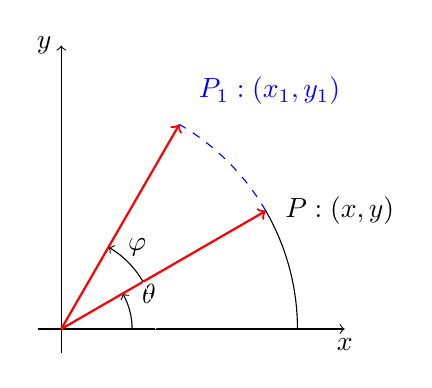
\begin{tikzpicture}[scale=3]
    % \draw[step=.5cm,gray,very thin] (-0.1,-0.1) grid (1.4,1.4);
    \draw[->] (-.1,0) -- (1.2,0)  node[below] {$x$};
    \draw[->] (0,-0.1) -- (0,1.2) node[left] {$y$};
    \draw[]   (1,0) arc (0:30:1) node(P)[label=right:$P:{(x,y)}$]{};
    \draw[->] (3mm,0mm) -- (3mm,0mm) arc (0:30:3mm) node(A)[label=right:$\theta$]{};
    \draw[red, thick, ->] (0,0) --  (P.center);
    
    \draw[white] (4mm,0mm) -- (4mm,0mm) arc (0:30:4mm) node(A){};
    \draw[->] (A.center) arc (30:60:4mm) node[label=right:$\varphi$]{};
    
    \draw[blue, dashed]  (P) arc (30:60:1) node(P1)[label=above right:$P_1:{(x_1,y_1)}$]{};
    
    \draw[red, thick, ->] (0,0) -- (P1.center);    
  \end{tikzpicture}
\end{figure}
这表明经过上述变换,将向量$OP$逆时针旋转$\varphi$角得到向量$OP_1$.


\begin{li}
  求解线性方程组
  $$
  \left\{
    \begin{array}{rcrcrcrcrr}
      2x_1 & - & 2x_2 &   &      & + &  6x_4 & = &-2 \\[0.1cm]
      2x_1 & - &  x_2 & + & 2x_3 & + &  4x_4 & = &-2 \\[0.1cm]
      3x_1 & - &  x_2 & + & 4x_3 & + &  4x_4 & = &-3 \\[0.1cm]
      5x_1 & - & 3x_2 & + &  x_3 & + & 20x_4 & = &-2 
    \end{array}
  \right.
  $$
\end{li}
\begin{jie}
  $$
  \left\{
    \begin{array}{rcrcrcrcrr}
      x_1 & - &  x_2 &   &      & + &  3x_4 & = &-1 \\[0.1cm]
          &  &  x_2 & + & 2x_3 & - &  2x_4 & = &0 \\[0.1cm]
          &  & 2x_2 & + & 4x_3 & - &  5x_4 & = &0 \\[0.1cm]
          &  & 2x_2 & + &  x_3 & + &  5x_4 & = &3 
    \end{array}
  \right.
  $$    
  $$
  \left\{
    \begin{array}{rcrcrcrcrr}
      x_1 & - &  x_2 &   &      & + &  3x_4 & = &-1 \\[0.1cm]
          &  &  x_2 & + & 2x_3 & - &  2x_4 & = &0 \\[0.1cm]
          &  &  &  &  & - &  x_4 & = &0 \\[0.1cm]
          &  &  & - &  3x_3 & + &  9x_4 & = &3 
    \end{array}
  \right.
  $$    
  $$
  \left\{
    \begin{array}{rcrcrcrcrr}
      x_1 & - &  x_2 &   &      & + &  3x_4 & = &-1 \\[0.1cm]
          &  &  x_2 & + & 2x_3 & - &  2x_4 & = &0 \\[0.1cm]
          &  &  & - &  3x_3 & + &  9x_4 & = &3 \\[0.1cm]
          &  &  &  &  & - &  x_4 & = &0 
    \end{array}
  \right.
  $$    
  $$
  \left\{
    \begin{array}{rcrcrcrcrr}
      x_1 & - &  x_2 &   &      & + &  3x_4 & = &-1 \\[0.1cm]
          &  &  x_2 & + & 2x_3 & - &  2x_4 & = &0 \\[0.1cm]
          &  &  &  &  x_3 & - &  3x_4 & = &-1 \\[0.1cm]
          &  &  &  &  &  &  x_4 & = &0 
    \end{array}
  \right.
  $$    
  如此形状的方程组称为\red{阶梯形线性方程组}.
  该方程组可写成矩阵形式
  \begin{figure}[htbp]
    \centering
    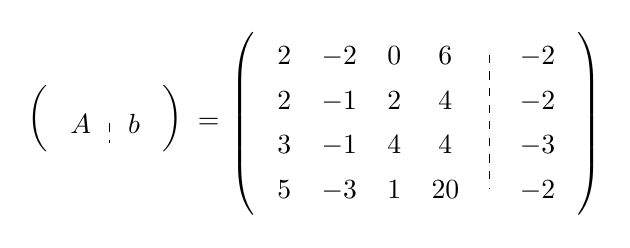
\begin{tikzpicture}
      \matrix(M) [matrix of math nodes,nodes in empty cells,,ampersand replacement=\&,left delimiter=(,right delimiter=)]{
        A \& \& b \\
      };
      \draw[dashed] (M-1-2.north) -- (M-1-2.south);
      \matrix(M1) [right=.1in of M,matrix of math nodes]{
        = \\
      };
      \matrix(MM) [right=.1in of M1,matrix of math nodes,nodes in empty cells,
      column sep=1ex,row sep=.5ex,ampersand replacement=\&,left delimiter=(,right delimiter=)] {
        2 \& -2 \& 0 \&  6 \& \& -2\\
        2 \& -1 \& 2 \&  4 \& \& -2\\
        3 \& -1 \& 4 \&  4 \& \& -3\\
        5 \& -3 \& 1 \& 20 \& \& -2\\
      };
      \draw[dashed] (MM-1-5.north) -- (MM-4-5);
    \end{tikzpicture}
    \caption{增广矩阵}
  \end{figure}
  求解过程可表示为
  \begin{figure}[htbp]
    \centering
    \begin{tikzpicture}          
      \matrix(A) [matrix of math nodes,nodes in empty cells,
      column sep=1ex,row sep=.1ex,ampersand replacement=\&,left delimiter=(,right delimiter=)] {
        A \& \& b \\
      };
      \draw[dashed] (A-1-2.north) -- (A-1-2.south);
      % \end{tikzpicture}
      
      % \begin{tikzpicture}
      \matrix (EQ1) [right=.1in of A,matrix of math nodes]  { 
        \xlongequal[]{\ds r_1 \div 2} \\
      };
      
      \matrix(A1) [right=.1in of EQ1,matrix of math nodes,nodes in empty cells, column sep=1ex,row sep=.1ex,ampersand replacement=\&,left delimiter=(,right delimiter=)] {
        1 \& -1 \& 0 \&  3 \& \& -1\\
        2 \& -1 \& 2 \&  4 \& \& -2\\
        3 \& -1 \& 4 \&  4 \& \& -3\\
        5 \& -3 \& 1 \& 20 \& \& -2\\
      };
      \draw[dashed] (A1-1-5.north) -- (A1-4-5);
      % \end{tikzpicture}

      
      % \begin{tikzpicture}
      
      \matrix(A2) [below=.1in of A1,matrix of math nodes,nodes in empty cells,
      column sep=1ex,row sep=.1ex,ampersand replacement=\&,left delimiter=(,right delimiter=)] {
        1 \& -1 \& 0 \&  3 \& \& -1\\
        0 \&  1 \& 2 \& -2 \& \&  0\\
        0 \&  0 \& 0 \& -1 \& \&  0\\
        0 \&  0 \&-3 \&  9 \& \&  3\\
      };
      \draw[dashed] (A2-1-5.north) -- (A2-4-5);
      \matrix (EQ2) [left=.1in of A2,matrix of math nodes]  { 
        \xlongequal[
        \ds r_3+(-3)\times r_1 \atop 
        \ds r_4+(-5)\times r_1]{\ds r_2+(-2)\times r_1} \\
      };

      % \end{tikzpicture}

      
      % \begin{tikzpicture}
      \matrix(A3) [below=.1in of A2,matrix of math nodes,nodes in empty cells,
      column sep=1ex,row sep=.1ex,ampersand replacement=\&,left delimiter=(,right delimiter=)] {
        1 \& -1 \& 0 \&  3 \& \& -1\\
        0 \&  1 \& 2 \& -2 \& \&  0\\
        0 \&  0 \&-3 \&  9 \& \&  3\\
        0 \&  0 \& 0 \& -1 \& \&  0\\
      };
      \draw[dashed] (A3-1-5.north) -- (A3-4-5);

      \matrix (EQ3) [left=.1in of A3,matrix of math nodes]  { 
        \xlongequal[]{\ds r_3 \leftrightarrow r_4} \\
      };

      
      \matrix(A4) [below=.1in of A3,matrix of math nodes,nodes in empty cells,
      column sep=1ex,row sep=.1ex,ampersand replacement=\&,left delimiter=(,right delimiter=)] {
        1 \& -1 \& 0 \&  3 \& \& -1\\
        0 \&  1 \& 2 \& -2 \& \&  0\\
        0 \&  0 \& 1 \& -3 \& \& -1\\
        0 \&  0 \& 0 \&  1 \& \&  0\\
      };
      \draw[dashed] (A4-1-5.north) -- (A4-4-5);

      \matrix (EQ4) [left=.1in of A4,matrix of math nodes]  { 
        \xlongequal[]{\ds r_3 \div (-3)} \\
      };
    \end{tikzpicture}
  \end{figure}
\end{jie}

\begin{li}
  求解线性方程组
  $$
  \left\{
    \begin{array}{rcrcrcrcrcrr}
      x_1 & - &  x_2 & - &  x_3 &   &       & + & 3x_5 & = &-1 \\[0.1cm]
      2x_1 & - & 2x_2 & - &  x_3 & + &  2x_4 & + & 4x_5 & = &-2 \\[0.1cm]
      3x_1 & - & 3x_2 & - &  x_3 & + &  4x_4 & + & 5x_5 & = &-3 \\[0.1cm]
      x_1 & - &  x_2 & + &  x_3 & + &   x_4 & + & 8x_5 & = & 2 
    \end{array}
  \right.
  $$
\end{li}
\newpage
\begin{jie}
  
  其增广矩阵为
  \begin{figure}[htbp]
    \centering
    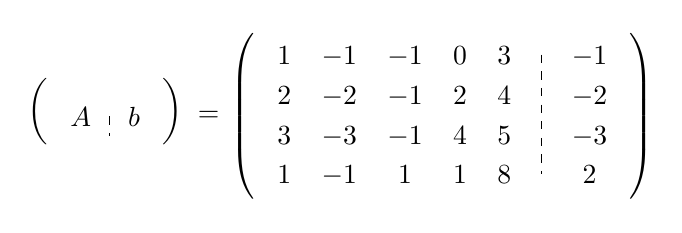
\begin{tikzpicture}
      \matrix(Ab) [matrix of math nodes,nodes in empty cells,,ampersand replacement=\&,left delimiter=(,right delimiter=)]{
        A \& \& b \\
      };
      \draw[dashed] (Ab-1-2.north) -- (Ab-1-2.south);
      \matrix (EQ) [right=.1in of Ab,matrix of math nodes]  { 
        =\\
      };
      \matrix(A) [right=.1in of EQ,matrix of math nodes,nodes in empty cells,   column sep=1ex,row sep=.1ex,ampersand replacement=\&,left delimiter=(,right delimiter=)] {
        1 \& -1 \& -1 \&  0 \& 3 \& \& -1\\
        2 \& -2 \& -1 \&  2 \& 4 \& \& -2\\
        3 \& -3 \& -1 \&  4 \& 5 \& \& -3\\
        1 \& -1 \&  1 \&  1 \& 8 \& \&  2\\
      };
      \draw[dashed] (A-1-6.north) -- (A-4-6);
    \end{tikzpicture}      
  \end{figure}
  
  求解过程可表示为:
  \begin{figure}[htbp]
    \centering
    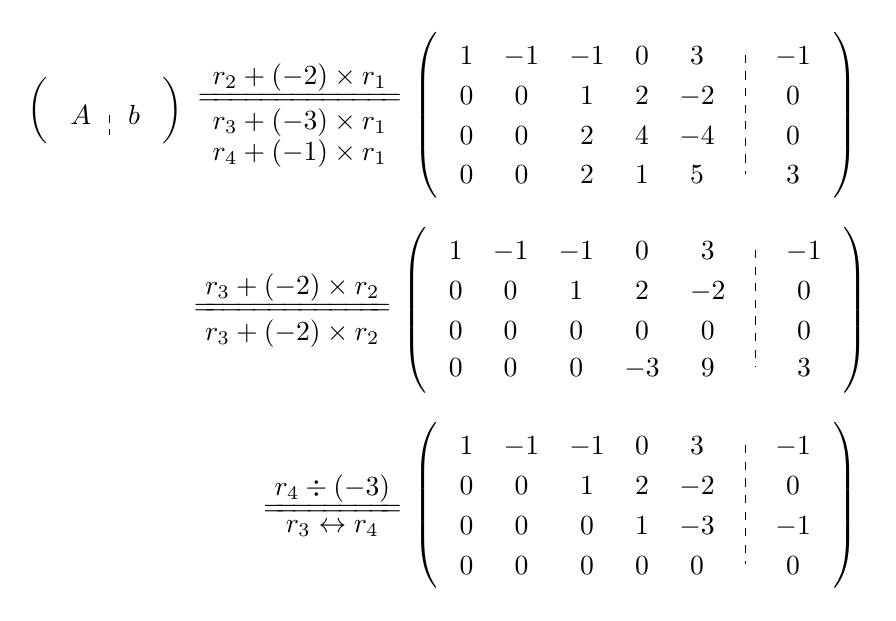
\begin{tikzpicture}
      \matrix(A) [matrix of math nodes,nodes in empty cells,,ampersand replacement=\&,left delimiter=(,right delimiter=)]{
        A \& \& b \\
      };
      \draw[densely dashed] (A-1-2.north) -- (A-1-2.south);
      \matrix (EQ1) [right=.1in of A,matrix of math nodes]  { 
        \xlongequal[\ds r_3+(-3)\times \ds r_1 \atop \ds r_4+(-1)\times r_1]{\ds r_2+(-2)\times r_1}\\
      };        
      \matrix(A1) [right=.1in of EQ1,matrix of math nodes,nodes in empty cells,
      column sep=1ex,row sep=.1ex,ampersand replacement=\&,left delimiter=(,right delimiter=)] {
        1 \& -1 \& -1 \&  0 \& 3 \& \& -1\\
        0 \&  0 \&  1 \&  2 \&-2 \& \&  0\\
        0 \&  0 \&  2 \&  4 \&-4 \& \&  0\\
        0 \&  0 \&  2 \&  1 \& 5 \& \&  3\\
      };
      \draw[dashed] (A1-1-6.north) -- (A1-4-6);

      \matrix(A2) [below=.1in of A1,matrix of math nodes,nodes in empty cells,
      column sep=1ex,row sep=.1ex,ampersand replacement=\&,left delimiter=(,right delimiter=)] {
        1 \& -1 \& -1 \&  0 \& 3 \& \& -1\\
        0 \&  0 \&  1 \&  2 \&-2 \& \&  0\\
        0 \&  0 \&  0 \&  0 \& 0 \& \&  0\\
        0 \&  0 \&  0 \& -3 \& 9 \& \&  3\\
      };
      \draw[dashed] (A2-1-6.north) -- (A2-4-6);
      \matrix (EQ2) [left=.1in of A2,matrix of math nodes]  { 
        \xlongequal[\ds r_3+(-2)\times r_2]{\ds r_3+(-2)\times r_2}\\
      };

      \matrix(A3) [below=.1in of A2,matrix of math nodes,nodes in empty cells,
      column sep=1ex,row sep=.1ex,ampersand replacement=\&,left delimiter=(,right delimiter=)] {
        1 \& -1 \& -1 \&  0 \& 3 \& \& -1\\
        0 \&  0 \&  1 \&  2 \&-2 \& \&  0\\
        0 \&  0 \&  0 \&  1 \& -3 \& \& -1\\
        0 \&  0 \&  0 \&  0 \& 0 \& \&  0\\
      };
      \draw[dashed] (A3-1-6.north) -- (A3-4-6);
      \matrix (EQ3) [left=.1in of A3,matrix of math nodes]  { 
        \xlongequal[\ds r_3 \leftrightarrow r_4]{\ds r_4\div(-3)}\\
      };
    \end{tikzpicture}           
  \end{figure}
  
  该矩阵称为\red{行简化阶梯矩阵},对应的线性方程组为
  $$
  \left\{
    \begin{array}{rcrcrcrcrcrr}
      x_1 & - &  x_2 &   &      &   &       & + & 7x_5 & = & 1 \\[0.1cm]
          &   &     &   &  x_3 &   &     & + & 4x_5 & = & 2 \\[0.1cm]
          &   &   &   &    &   &   x_4 & - & 3x_5 & = &-1
    \end{array}
  \right.
  $$
  \begin{zhu}
    该方程组有$5$个未知量,其中$x_1,x_3,x_4$为\red{基本未知量},$x_2,x_5$为\red{自由未知量}。
  \end{zhu}

  任取$x_2=k_1, x_5=k_2$,可得线性方程组的全部解
  $$
  \left\{
    \begin{array}{ccl}
      x_1 &=& 1+k_1-7k_2, \\[0.1cm]      
      x_2 &=& k_1, \\[0.1cm]
      x_3 &=& 2-4k_2, \\[0.1cm]
      x_4 &=& -1+3k_2,\\[0.1cm]
      x_5 &=& k_2.
    \end{array}
  \right.
  $$

\end{jie}

\begin{li}
  解线性方程组
  $$
  \left\{
    \begin{array}{rcrcrcr}
      x_1 & + & x_2 & + &  x_3 & = & 1, \\[0.1cm]
      x_1 & + &2x_2 & - & 5x_3 & = & 2, \\[0.1cm]
      2x_1 & + &3x_2 & - & 4x_3 & = & 5.
    \end{array}
  \right.
  $$
\end{li}
\newpage
\begin{jie}
  
  \begin{figure}[htbp]
    \centering
    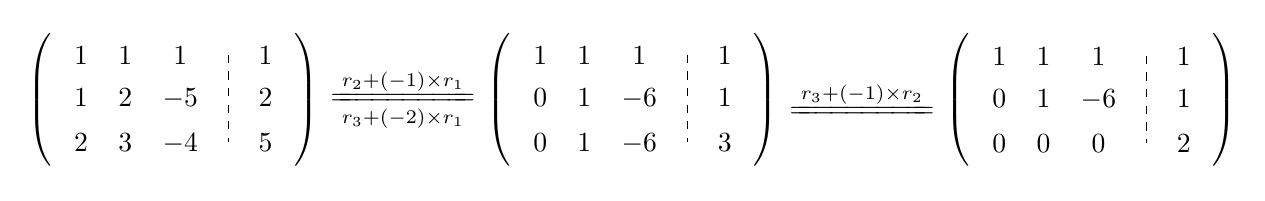
\begin{tikzpicture}        
      \matrix(Ab) [matrix of math nodes,nodes in empty cells,
      column sep=1ex,row sep=.5ex,ampersand replacement=\&,left delimiter=(,right delimiter=)] {
        1 \&  1 \&  1 \& \&  1\\
        1 \&  2 \& -5 \& \&  2\\
        2 \&  3 \& -4 \& \&  5\\
      };
      \draw[dashed] (Ab-1-4.north) -- (Ab-3-4);
      
      \matrix (EQ1) [right=.1in of Ab,matrix of math nodes]  { 
        \xlongequal[r_3+ (-2)\times r_1]{r_2+ (-1)\times r_1}\\
      };

      \matrix(Ab1) [right=.1in of EQ1,matrix of math nodes,nodes in empty cells, column sep=1ex,row sep=.5ex,ampersand replacement=\&,left delimiter=(,right delimiter=)] {
        1 \&  1 \&  1 \& \&  1\\
        0 \&  1 \& -6 \& \&  1\\
        0 \&  1 \& -6 \& \&  3\\
      };
      \draw[dashed] (Ab1-1-4.north) -- (Ab1-3-4);

      \matrix (EQ2) [right=.1in of Ab1,matrix of math nodes]  { 
        \xlongequal[]{r_3+ (-1)\times r_2}\\
      };
      \matrix(Ab2) [right=.1in of EQ2,matrix of math nodes,nodes in empty cells,column sep=1ex,row sep=.5ex,ampersand replacement=\&,left delimiter=(,right delimiter=)] {
        1 \&  1 \&  1 \& \&  1\\
        0 \&  1 \& -6 \& \&  1\\
        0 \&  0 \&  0 \& \&  2\\
      };
      \draw[dashed] (Ab2-1-4.north) -- (Ab2-3-4);        
    \end{tikzpicture}
  \end{figure}
  
  由第三行可以看出,该线性方程组无解。
\end{jie}

\begin{itemize}
\item 含有矛盾方程而无解的方程组称为\red{不相容方程组};
\item 有解的方程组称为\red{相容方程组};
\item \red{多余方程}。
\end{itemize}

对于一般的线性方程组
$$
\left\{
  \begin{array}{c}
    a_{11}x_1 + a_{12}x_2 + \cd + a_{1n}x_n = b_1\\[0.2cm]
    a_{21}x_1 + a_{22}x_2 + \cd + a_{2n}x_n = b_2\\[0.2cm]
    \vd\\[0.2cm]
    a_{m1}x_1 + a_{m2}x_2 + \cd + a_{mn}x_n = b_m
  \end{array}
\right.
$$

其增广矩阵为
\begin{figure}[htbp]
  \centering
  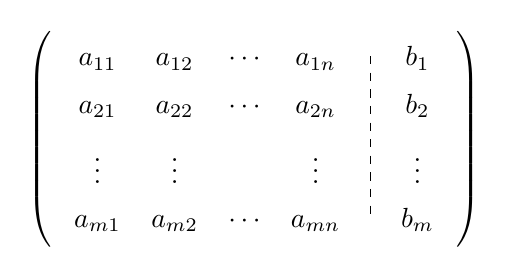
\begin{tikzpicture}
    \matrix(MM) [matrix of math nodes,nodes in empty cells,
    column sep=1ex,row sep=.5ex,ampersand replacement=\&,left delimiter=(,right delimiter=)] {
      a_{11} \&  a_{12} \&  \cd \& a_{1n} \& \&  b_1\\
      a_{21} \&  a_{22} \&  \cd \& a_{2n} \& \&  b_2\\
      \vd   \&  \vd   \&      \&  \vd  \& \& \vd \\
      a_{m1} \&  a_{m2} \&  \cd \& a_{mn} \& \&  b_m\\
    };
    \draw[dashed] (MM-1-5.north) -- (MM-4-5);        
  \end{tikzpicture}      
\end{figure}
对于以上增广矩阵,总是可以经过一系列的变换将其化成
\begin{figure}[htbp]
  \centering
  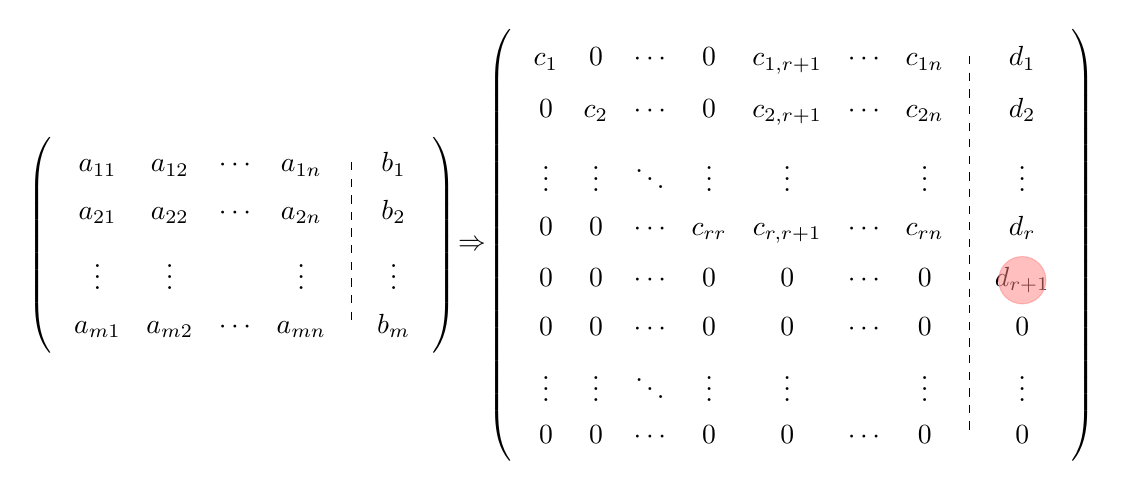
\begin{tikzpicture}
    \matrix(MM) [matrix of math nodes,nodes in empty cells,
    column sep=0.6ex,row sep=.5ex,ampersand replacement=\&,left delimiter=(,right delimiter=)] {
      a_{11} \&  a_{12} \&  \cd \& a_{1n} \& \&  b_1\\
      a_{21} \&  a_{22} \&  \cd \& a_{2n} \& \&  b_2\\
      \vd   \&  \vd   \&      \&  \vd  \& \& \vd \\
      a_{m1} \&  a_{m2} \&  \cd \& a_{mn} \& \&  b_m\\
    };
    \draw[dashed] (MM-1-5.north) -- (MM-4-5);
    
    \matrix (M2) [right=.05in of MM,matrix of math nodes]  { 
      \Rightarrow\\
    };
    
    \matrix(MM) [right=.05in of M2,matrix of math nodes,nodes in empty cells,
    column sep=0.6ex,row sep=.5ex,ampersand replacement=\&,left delimiter=(,right delimiter=)] {
      c_1 \&   0 \& \cd \&  0 \& c_{1,r+1} \& \cd \& c_{1n} \& \& d_1\\
      0   \& c_2 \& \cd \&  0 \& c_{2,r+1} \& \cd \& c_{2n} \& \& d_2\\
      \vd \& \vd \& \dd \&\vd \& \vd     \&     \& \vd   \& \& \vd\\
      0   \&  0  \& \cd \& c_{rr} \& c_{r,r+1} \& \cd \& c_{rn} \& \& d_r\\
      0   \&  0  \& \cd \& 0 \& 0 \& \cd \& 0 \&  \& d_{r+1}\\
      0   \&  0  \& \cd \& 0 \& 0 \& \cd \& 0 \&  \& 0\\          
      \vd \& \vd \& \dd \&\vd \& \vd     \&     \& \vd   \& \& \vd\\
      0   \&  0  \& \cd \& 0 \& 0 \& \cd \& 0 \&  \& 0\\
    };
    \draw[dashed] (MM-1-8.north) -- (MM-8-8);
    \filldraw[opacity=0.5,red!50] (MM-5-9) circle (0.3cm);
  \end{tikzpicture}      
\end{figure}
其中$c_{ii}=1~(i=1,2,\cd,r)$。对应线性方程组解的情况如下:   
\begin{itemize}
\item[1] 线性方程组有解$ \Leftrightarrow \red{d_{r+1}=0}$;\\[0.3cm]
\item[2] 在有解的情况下:
  \begin{itemize}
  \item 当$r=n$时,有唯一解$x_1=d_1,~x_2=d_2,~\cd,~x_n=d_n$;
  \item 当$r<n$时,有无穷多解
    $$
    \left\{
      \begin{array}{ccl}
        x_1 &=& d_1 - c_{1,r+1}k_1 - \cd - c_{1n}k_{n-r}, \\[0.1cm]
        x_2 &=& d_2 - c_{2,r+1}k_1 - \cd - c_{2n}k_{n-r}, \\[0.1cm]
        \vd & & \vd \\[0.1cm]
        x_r &=& d_r - c_{r,r+1}k_1 - \cd - c_{rn}k_{n-r}, \\[0.1cm]
        x_{r+1} &=& k_1, \\[0.1cm]
        \vd && \vd \\[0.1cm]
        x_{n} &=& k_{n-r}.
      \end{array}
    \right.
    $$
  \end{itemize}
\end{itemize}

\section{行列式的性质}

\begin{frame}
\begin{xingzhi}
  互换行列式的行与列,值不变。即
  \begin{equation}
    \left|
      \begin{array}{cccc}
        a_{11}  &  a_{12} & \cdots & a_{1n} \\
        a_{21}  &  a_{22} & \cdots & a_{2n} \\
        \vdots & \vdots & \ddots & \vdots\\  
        a_{n1}  &  a_{n2} & \cdots & a_{nn} 
      \end{array}
    \right|
    =
    \left|
      \begin{array}{cccc}
        a_{11}  &  a_{21} & \cdots & a_{n1} \\
        a_{12}  &  a_{22} & \cdots & a_{n2} \\
        \vdots & \vdots & \ddots & \vdots\\  
        a_{1n}  &  a_{2n} & \cdots & a_{nn} 
      \end{array}
    \right|
  \end{equation}
\end{xingzhi}
\end{frame}

\begin{frame} 
\blue{\proofname.~}  
  将等式两端的行列式分别记为$D$和$D^\prime$,对阶数$n$用归纳法。\pause 
  
  \noindent(1) 当$n=2$时,$D=D^\prime$显然成立。  \\[0.1in] \pause 
  \noindent(2) 假设结论对于阶数小于$n$的行列式都成立,以下考虑阶数为$n$的情况。由定义可知,
    $$
    \begin{array}{c}
      D = a_{11} A_{11}+a_{12}A_{12}+\cdots+a_{1n}A_{1n}, \\[0.1in]
      D^\prime = a_{11} A^\prime_{11}+a_{21}A^\prime_{21}+\cdots+a_{n1}A^\prime_{n1}
    \end{array}
    $$
    显然,$A_{11}=A^\prime_{11}$。
 

\end{frame}

\begin{frame}
于是
$$
\begin{aligned}
D^\prime =&
a_{11} A_{11}+(-1)^{1+2}a_{21}
\left|
\begin{array}{cccc}
a_{12} & a_{32} & \cdots & a_{n2} \\
a_{13} & a_{33} & \cdots & a_{n3} \\
\vdots & \vdots & & \vdots \\
a_{1n} & a_{3n} & \cdots & a_{nn} \\
\end{array}
\right|  \\
&+ (-1)^{1+3}a_{31}
\left|
\begin{array}{ccccc}
a_{12} & a_{22} & a_{42} & \cdots & a_{n2} \\
a_{13} & a_{23} & a_{43} & \cdots & a_{n3} \\
\vdots & \vdots & \vdots & & \vdots \\
a_{1n} & a_{2n} & a_{4n} & \cdots & a_{nn} \\
\end{array}
\right|  \\
& + \cdots + (-1)^{1+n} a_{n1} \left|
\begin{array}{cccc}
a_{12} & a_{22} & \cdots & a_{n-1,2} \\
a_{13} & a_{23} & \cdots & a_{n-1,3} \\
\vdots & \vdots & & \vdots \\
a_{1n} & a_{2n} & \cdots & a_{n-1,n} \\
\end{array}
\right|
\end{aligned}
$$
\end{frame}

\begin{frame}
    对上式中的$n-1$个行列式按第一行展开,并将含$a_{12}$的项进行合并,可得
    $$
    \begin{aligned}
      & (-1)^{1+2}a_{21} a_{12}
      \left|
        \begin{array}{ccc}       
          a_{33} & \cdots & a_{n3} \\
          \vdots  & & \vdots \\
          a_{3n} & \cdots & a_{nn} \\
        \end{array}
      \right| 
      + (-1)^{1+3}a_{31} a_{12}
      \left|
        \begin{array}{cccc}
          a_{23}  & a_{43} & \cdots & a_{n3} \\
          \vdots & \vdots & & \vdots \\
          a_{2n}  & a_{4n} & \cdots & a_{nn} \\
        \end{array}
      \right|  \\
      & \hspace{1in} + \cdots +(-1)^{1+n} a_{n1} a_{12}
      \left|
        \begin{array}{ccc}
          a_{23} & \cdots & a_{n-1,3} \\
          \vdots & & \vdots \\
          a_{2n} & \cdots & a_{n-1,n} \\
        \end{array}
      \right|\\
      = &   -a_{12} \left(
        (-1)^{1+1} a_{21} 
        \left|
          \begin{array}{ccc}       
            a_{33} & \cdots & a_{n3} \\
            \vdots  & & \vdots \\
            a_{3n} & \cdots & a_{nn} \\
          \end{array}
        \right|    
        + (-1)^{1+2}a_{31} 
        \left|
          \begin{array}{cccc}
            a_{23}  & a_{43} & \cdots & a_{n3} \\
            \vdots & \vdots & & \vdots \\
            a_{2n}  & a_{4n} & \cdots & a_{nn} \\
          \end{array}
        \right|\right.\\
      &  \hspace{1in} \left. + \cdots + (-1)^{1+n-1} a_{n1}
        \left|
          \begin{array}{ccc}
            a_{23} & \cdots & a_{n-1,3} \\
            \vdots & & \vdots \\
            a_{2,n} & \cdots & a_{n-1,n} \\
          \end{array}
        \right|
      \right)\\
      % =  (-1)^{1+2} a_{12} \left(      
      %   \left|
      %     \begin{array}{cccc}       
      %       a_{21} & 0 & \cdots & 0 \\
      %       0 & a_{33} & \cdots & a_{n3} \\
      %       0 & \vdots  & & \vdots \\
      %       0 & a_{3n} & \cdots & a_{nn} \\
      %     \end{array}
      %   \right|  
      %   + 
      %   \left|
      %     \begin{array}{ccccc}
      %       0 & a_{31} & 0 & \cdots & 0 \\
      %       a_{23}  & 0 & a_{43} & \cdots & a_{n3} \\
      %       \vdots & 0 & \vdots & & \vdots \\
      %       a_{2n}  & 0 & a_{4n} & \cdots & a_{nn} \\
      %     \end{array}
      %   \right|  \right.\\
      % + \cdots + \left. 
      %   \left|
      %     \begin{array}{cccc}
      %       0 & \cdots & 0 & a_{n-1} \\
      %       a_{23} & \cdots & a_{n-1,3} & 0 \\
      %       \vdots & & \vdots & 0\\
      %       a_{2,n3} & \cdots & a_{n-1,n} & 0 \\
      %     \end{array}
      %   \right|
      % \right)\\
      = &- a_{12}
      \left|
        \begin{array}{cccc}
          a_{21} & a_{31} & \cdots & a_{n1} \\
          a_{23} & a_{33} & \cdots & a_{n3} \\
          \vdots & \vdots & & \vdots \\
          a_{2n} & a_{3n} & \cdots & a_{nn}        
        \end{array}
      \right| = -a_{12} M_{12}^\prime  = a_{12} A_{12}^\prime = a_{12} A_{12}. 
    \end{aligned}
    $$
\end{frame}

\begin{frame}
    同理,含$a_{13}$的项合并后其值等于$a_{13}A_{13}$,$\cdots$,
    含$a_{1n}$的项合并后其值等于$a_{1n}A_{1n}$. 因此,$D=D^\prime$.  \qed

 

\end{frame}

\begin{frame}
\begin{zhu}
  有了这个性质,行列式对行成立的性质都适用于列。
\end{zhu}
\end{frame}

\begin{frame}
\begin{xingzhi}
  行列式对任一行按下式展开,其值相等,即
  $$
  D = a_{i1} A_{i1} + a_{i2} A_{i2} + \cdots + a_{in}A_{in} = \sum_{j=1}^n a_{ij} A_{ij}, \quad
  i = 1, 2, \cdots, n,
  $$
  其中
  $$
  A_{ij} = (-1)^{i+j} M_{ij}
  $$
  而$M_{ij}$为$a_{ij}$的余子式,$A_{ij}$为$a_{ij}$的代数余子式.
\end{xingzhi}
\end{frame}

\begin{frame}
\blue{\proofname.}~ 
  对$n$用归纳法证明。 \\[0.1in]\pause
  
  \noindent (1) 当$n=2$时,结论显然成立。\\[0.1in]\pause
  \noindent (2) 假设结论对阶数$\le n-1$的行列式成立,以下考虑阶数为$n$的情况。
    $$
    \begin{aligned}
      D = &  (-1)^{2} a_{11} \left|
        \begin{array}{cccc}
          a_{22}  & a_{23}   & \cdots & a_{2n}\\
          \vdots  & \vdots & & \vdots \\
          a_{i2}  & a_{i3}   & \cdots & a_{in}\\
          \vdots & \vdots  & & \vdots \\
          a_{n2}  & a_{n3}   & \cdots & a_{nn}\\
        \end{array}
      \right|_{n-1} + (-1)^{3} a_{12} \left|
        \begin{array}{cccc}
          a_{21}  & a_{23}  & \cdots & a_{2n}\\
          \vdots & \vdots & & \vdots \\
          a_{i1}  & a_{i3}  & \cdots & a_{in}\\
          \vdots & \vdots & & \vdots \\
          a_{n1}  & a_{n3}  & \cdots & a_{nn}\\
        \end{array}
      \right|_{n-1}\\
      & 
%      + (-1)^{1+3} a_{13} \left|
%        \begin{array}{ccccc}
%          a_{21}  & a_{22} & a_{24}  & \cdots & a_{2n}\\
%          \vdots & \vdots & \vdots & & \vdots \\
%          a_{i1}  & a_{i2} & a_{24}  & \cdots & a_{in}\\
%          \vdots & \vdots & \vdots & & \vdots \\
%          a_{n1}  & a_{n2}  & a_{n4} & \cdots & a_{nn}\\
%        \end{array}
%      \right|_{n-1}
      + \cdots  
      + (-1)^{1+n} a_{n+1} \left|
        \begin{array}{cccc}
          a_{21}  & a_{22}   & \cdots & a_{2,n-1}\\
          \vdots  & \vdots & & \vdots \\
          a_{i1}  & a_{i2}   & \cdots & a_{i,n-1}\\
          \vdots & \vdots  & & \vdots \\
          a_{n1}  & a_{n2}   & \cdots & a_{n,n-1}\\
        \end{array}
      \right|_{n-1}
    \end{aligned}
    $$
\end{frame}

\begin{frame}    
    由归纳假设,将上式中的所有$n-1$阶行列式按第$i$行展开后合并含$a_{i1}$的项得,
    $$
    \begin{aligned}
      (-1)^{i+1}a_{i1}  & \left (  (-1)^{1+1} a_{12}  \left|
          \begin{array}{cccc}
            a_{23}  & a_{24}  & \cdots & a_{2n}\\
            \vdots & \vdots & & \vdots \\
            a_{i-1,3}  & a_{i-1,4}  & \cdots & a_{i-1,n}\\
            a_{i+1,3}  & a_{i+1,4}  & \cdots & a_{i+1,n}\\
            \vdots & \vdots & & \vdots \\
            a_{n,3}  & a_{n,4}  & \cdots & a_{nn}
          \end{array}
        \right|_{n-2} \right. \\
        & + (-1)^{1+2} a_{13}   \left|
          \begin{array}{cccc}
            a_{22} & a_{24}  & \cdots & a_{2n}\\
            \vdots & \vdots & & \vdots \\
            a_{i-1,2} & a_{i-1,4}  & \cdots & a_{i-1,n}\\
            a_{i+1,2} & a_{i+1,4}  & \cdots & a_{i+1,n}\\
            \vdots & \vdots & & \vdots \\
            a_{n2}  & a_{n4} & \cdots & a_{nn}
          \end{array}
        \right|_{n-2}+ \cdots
       \\
      & \left.   +  (-1)^{1+(n-1)} a_{1n}  \left|
          \begin{array}{ccc}
            a_{22}   & \cdots & a_{2,n-1}\\
            \vdots & & \vdots \\
            a_{i-1,2}   & \cdots & a_{i-1,n-1}\\
            a_{i+1,2}   & \cdots & a_{i+1,n-1}\\
            \vdots  & & \vdots \\
            a_{n2}   & \cdots & a_{n,n-1}
          \end{array}
        \right|_{n-2} \right) 
    \end{aligned}
    $$
\end{frame}

\begin{frame} 
    即
    $$
    (-1)^{i+1}a_{i1} \left|
      \begin{array}{cccc}
        a_{12} & a_{13} & \cdots & a_{1n} \\
        a_{22} & a_{23} & \cdots & a_{2n}\\
        \vdots & \vdots & & \vdots \\
        a_{i-1,2} & a_{i-1,3}   & \cdots & a_{i-1,n}\\    
        a_{i-1,2} & a_{i-1,3}   & \cdots & a_{i-1,n}\\
        \vdots & \vdots & & \vdots \\
        a_{n2}  & a_{n3} & \cdots & a_{nn}
      \end{array}
    \right| = (-1)^{i+1}a_{i1} M_{i1} = a_{i1} A_{i1}.
    $$
    同理可证,含$a_{i2}$的项合并后其值为$a_{i2}A_{i2}$,$\cdots$,含$a_{in}$的项合并后其值为$a_{in}A_{in}$.  
 
\end{frame}

\begin{frame} 

\begin{xingzhi}[线性性质]
  \begin{itemize}
  \item[1] 行列式的某一行(列)中所有的元素都乘以同一个数$k$,等于用数$k$乘以此行列式,即
    \begin{equation}\label{xz3-1}
      \left|
        \begin{array}{ccccc}
          a_{11}  & a_{12} & \cdots & a_{1n} \\
          \vdots & \vdots     &        & \vdots \\
          ka_{i1}  & ka_{i2} & \cdots & ka_{in} \\
          \vdots & \vdots     &        & \vdots \\
          a_{n1}  & a_{n2} & \cdots & a_{nn}
        \end{array}
      \right| = k
      \left|
        \begin{array}{ccccc}
          a_{11}  & a_{12} & \cdots & a_{1n} \\
          \vdots & \vdots     &        & \vdots \\
          a_{i1}  & a_{i2} & \cdots & a_{in} \\
          \vdots & \vdots     &        & \vdots \\
          a_{n1}  & a_{n2} & \cdots & a_{nn}
        \end{array}
      \right|
    \end{equation}
  \item[2] 若行列式的某一行(列)的元素都是两数之和,如       \begin{equation}\label{xz3-2}
      \begin{aligned}
        \left|
        \begin{array}{ccccc}
          a_{11} & \cdots & a_{1j}+b_{1j} & \cdots & a_{1n} \\
          a_{21} & \cdots & a_{2j}+b_{2j} & \cdots & a_{2n} \\
          \vdots&        & \vdots      &        & \vdots \\
          a_{n1} & \cdots & a_{nj}+b_{nj} & \cdots & a_{nn}
        \end{array}
        \right| & =  
        \left|
    \begin{array}{ccccc}
      a_{11} & \cdots & a_{1j} & \cdots & a_{1n} \\
      a_{21} & \cdots & a_{2j} & \cdots & a_{2n} \\
      \vdots&        & \vdots      &        & \vdots \\
      a_{n1} & \cdots & a_{nj} & \cdots & a_{nn}
    \end{array}                                                                                        \right|\\ 
    &+ \left| 
    \begin{array}{ccccc}
    a_{11} & \cdots & b_{1j} & \cdots & a_{1n} \\
    a_{21} & \cdots & b_{2j} & \cdots & a_{2n} \\
    \vdots&        & \vdots      &        & \vdots \\
    a_{n1} & \cdots & b_{nj} & \cdots & a_{nn}                                                                                                        \end{array}
                                                                                                                                               \right|          
      \end{aligned}
    \end{equation}
  \end{itemize}
\end{xingzhi}

\end{frame}

\begin{frame} 
\begin{zhu}一些记号:
  \begin{itemize}
  \item $r_i\times k$($c_i\times k$):第$i$行(列)乘以$k$
  \item $r_i\div k$($c_i\div k$):第$i$行(列)提取公因子$k$
  \end{itemize}
\end{zhu}

\end{frame}

\begin{frame} 
\begin{dingyi}[反对称行列式]
  如果行列式$D=|a_{ij}|_{n}$的元素满足
  $$
  a_{ij}=-a_{ji}(i,j=1,2,\cdots,n)
  $$
  就称$D$是\red{反对称行列式}。其中
  $$
  a_{ii}=-a_{ii}\Rightarrow a_{ii}=0.
  $$
\end{dingyi}
\end{frame}

\begin{frame}

\begin{li}
  证明:奇数阶反对称行列式的值为$0$.
\end{li} \pause
\begin{proof}
  $$
  \begin{aligned}
    D &= \left|
      \begin{array}{cccc}
        0 & a_{12} & \cd & a_{1n} \\
        -a_{12} & 0 & \cd & a_{2n} \\
        \vd & \vd & \dd & \vd \\
        -a_{1n} & -a_{2n} & \cd & 0
      \end{array}
    \right|
    \xlongequal[]{\text{性质1}}   \left|
      \begin{array}{cccc}
        0 & -a_{12} & \cd & -a_{1n} \\
        a_{12} & 0 & \cd & -a_{2n} \\
        \vd & \vd & \dd & \vd \\
        a_{1n} & a_{2n} & \cd & 0
      \end{array}
    \right| \\
    &  \xlongequal[\text{将每行提取公因子$-1$}]{\text{性质3-1}} 
    (-1)^n \left|
      \begin{array}{cccc}
        0 & a_{12} & \cd & a_{1n} \\
        -a_{12} & 0 & \cd & a_{2n} \\
        \vd & \vd & \dd & \vd \\
        -a_{1n} & -a_{2n} & \cd & 0
      \end{array}
    \right| = (-1)^n D.
  \end{aligned}  
  $$
  由于$n$为奇数,故$D=-D$,从而$D=0$.
\end{proof}
\end{frame}

\begin{frame}
\begin{tuilun}
  若行列式的某行元素全为0,其值为0.
\end{tuilun} \pause 


\begin{li}
  $$
  \left|
    \begin{array}{ccc}
      1 & 2 & 3\\
      0 & 0 & 0\\
      2 & 5 & 1
    \end{array}
  \right| = 0.
  $$
\end{li}
\end{frame}

\begin{frame}

\begin{xingzhi}
  若行列式有两行(列)完全相同,其值为$0$.
\end{xingzhi} \pause 

\begin{li}
	$$
	\left|
	\begin{array}{ccc}
	1 & 2 & 3\\
	1 & 2 & 3\\
	2 & 3 & 4
	\end{array}
	\right| = 0.
	$$
\end{li}

\end{frame}

\begin{frame} 
\begin{proof}
  不妨设$D$的第$i$和$j$行元素全部相等,即对
  $$
  D = \left|
    \begin{array}{cccc}
      a_{11}  &  a_{12} & \cdots & a_{1n} \\
      \vdots & \vdots &  & \vdots\\  
      a_{i1}  &  a_{i2} & \cdots & a_{in} \\
      \vdots & \vdots &  & \vdots\\  
      a_{j1}  &  a_{j2} & \cdots & a_{jn} \\
      \vdots & \vdots &  & \vdots\\  
      a_{n1}  &  a_{n2} & \cdots & a_{nn} 
    \end{array}
  \right|,
  $$
  有$a_{il}=a_{jl}(i\ne j, l=1,2,\cdots,n)$.
  对阶数$n$用数学归纳法。 \pause 
  \begin{itemize}
  \item 当$n=2$时,结论显然成立。\pause 
  \item 假设结论对阶数为$n-1$的行列式成立,在$n$阶的情况下,对第$k(k\ne i, j)$行展开,有
    $$
    D = a_{k1} A_{k1} + a_{k2} A_{k2} + \cdots + a_{kn} A_{kn}. 
    $$  \pause 
    注意到余子式$M_{kl}(l=1,2,\cdots,n)$是$n-1$阶行列式,且其中有两行元素相同,故
    $$
    A_{kl} = (-1)^{k+l} M_{kl} = 0\quad (l=1,2,\cdots,n),
    $$
    从而$D=0$.
  \end{itemize}
\end{proof}
\end{frame}

\begin{frame} 

%
\begin{tuilun}
  若行列式中有两行(列)元素成比例,则行列式的值为$0$.
\end{tuilun} \pause 
\begin{li}
  $$
  \left|
    \begin{array}{ccc}
      2 & 0 & -2\\
      1 & 0 & -1\\
      2 & 3 & 4
    \end{array}
  \right| =2 \left|
    \begin{array}{ccc}
      1 & 0 & -1\\
      1 & 0 & -1\\
      2 & 3 & 4
    \end{array}
  \right| = 0.
  $$
\end{li}
%
\end{frame}

\begin{frame}
\begin{xingzhi}
  把行列式的某一行(列)的各元素乘以同一个数然后加到另一行(列)对应的元素上去,行列式的值不变。
\end{xingzhi} \pause 
\begin{proof}
  将数$k$乘以第$j$行加到第$i$行,有
  $$
  \begin{aligned}
  & \left|
  \begin{array}{cccc}
    a_{11} & a_{12} & \cdots & a_{1n}\\
    \vdots & \vdots &  & \vdots \\
    a_{i1}+k a_{j1} & a_{i2}+k a_{j2} & \cdots & a_{in}+k a_{jn}\\
    \vdots & \vdots &  & \vdots \\
    a_{j1} & a_{j2} & \cdots & a_{jn}\\
    \vdots & \vdots &  & \vdots \\
    a_{n1} & a_{n2} & \cdots & a_{nn}
  \end{array}
  \right| \pause \xlongequal[]{\text{性质3-2}}   \blue{\left|
  \begin{array}{cccc}
  a_{11} & a_{12} & \cdots & a_{1n}\\
  \vdots & \vdots &  & \vdots \\
  a_{i1} & a_{i2} & \cdots & a_{in}\\
  \vdots & \vdots &  & \vdots \\
  a_{j1} & a_{j2} & \cdots & a_{jn}\\
  \vdots & \vdots &  & \vdots \\
  a_{n1} & a_{n2} & \cdots & a_{nn}
  \end{array}
  \right|} \\
  &\hspace{1in}\blue{+
  \left|
  \begin{array}{cccc}
  a_{11} & a_{12} & \cdots & a_{1n}\\
  \vdots & \vdots &  & \vdots \\
  k a_{j1} & k a_{j2} & \cdots & k a_{jn}\\
  \vdots & \vdots &  & \vdots \\
  a_{j1} & a_{j2} & \cdots & a_{jn}\\
  \vdots & \vdots &  & \vdots \\
  a_{n1} & a_{n2} & \cdots & a_{nn}
  \end{array}
  \right|}\pause \xlongequal[]{\text{推论2}}  
  \left|
  \begin{array}{cccc}
  a_{11} & a_{12} & \cdots & a_{1n}\\
  \vdots & \vdots &  & \vdots \\
  a_{i1} & a_{i2} & \cdots & a_{in}\\
  \vdots & \vdots &  & \vdots \\
  a_{j1} & a_{j2} & \cdots & a_{jn}\\
  \vdots & \vdots &  & \vdots \\
  a_{n1} & a_{n2} & \cdots & a_{nn}
  \end{array}
  \right|
  \end{aligned}
  $$
\end{proof}
\end{frame}

\begin{frame}
\begin{zhu}一些记号:
  \begin{itemize}
  \item $r_i + r_j\times k$:将第$j$行乘以$k$加到第$i$行;
  \item $c_i + c_j\times k$:将第$j$列乘以$k$加到第$i$列。 
  \end{itemize}

\end{zhu}
%
\end{frame}

\begin{frame}
\begin{xingzhi}
  互换行列式的两行(列),行列式变号。
\end{xingzhi} \pause 
\begin{proof}
  $$
  \begin{aligned}
    D &= \left|
      \begin{array}{cccc}
        a_{11} & a_{12} & \cdots & a_{1n}\\
        \vdots & \vdots &  & \vdots \\
        a_{i1} & a_{i2} & \cdots & a_{in}\\
        \vdots & \vdots &  & \vdots \\
        a_{j1} & a_{j2} & \cdots & a_{jn}\\
        \vdots & \vdots &  & \vdots \\
        a_{n1} & a_{n2} & \cdots & a_{nn}
      \end{array}
    \right| \xlongequal[r_i+r_j]{\text{性质5}} 
    \left|
      \begin{array}{cccc}
        a_{11} & a_{12} & \cdots & a_{1n}\\
        \vdots & \vdots &  & \vdots \\
        a_{i1}+a_{j1} & a_{i2}+a_{j2} & \cdots & a_{in}+a_{jn}\\
        \vdots & \vdots &  & \vdots \\
        a_{j1} & a_{j2} & \cdots & a_{jn}\\
        \vdots & \vdots &  & \vdots \\
        a_{n1} & a_{n2} & \cdots & a_{nn}
      \end{array}
    \right|\\[0.1in]
    &\xlongequal[r_j-r_i]{\text{性质5}} 
    \left|
      \begin{array}{cccc}
        a_{11} & a_{12} & \cdots & a_{1n}\\
        \vdots & \vdots &  & \vdots \\
        a_{i1}+a_{j1} & a_{i2}+a_{j2} & \cdots & a_{in}+a_{jn}\\
        \vdots & \vdots &  & \vdots \\
        -a_{i1} & -a_{i2} & \cdots & -a_{in}\\
        \vdots & \vdots &  & \vdots \\
        a_{n1} & a_{n2} & \cdots & a_{nn}
      \end{array}
    \right|
    \xlongequal[r_i+r_j]{\text{性质5}} 
    \left|
      \begin{array}{cccc}
        a_{11} & a_{12} & \cdots & a_{1n}\\
        \vdots & \vdots &  & \vdots \\
        a_{j1} & a_{j2} & \cdots & a_{jn}\\
        \vdots & \vdots &  & \vdots \\
        -a_{i1} & -a_{i2} & \cdots & -a_{in}\\
        \vdots & \vdots &  & \vdots \\
        a_{n1} & a_{n2} & \cdots & a_{nn}
      \end{array}
    \right| \\[0.1in]
    &\xlongequal[]{\text{性质3-1}} - D.
  \end{aligned}
  $$
\end{proof}
\end{frame}

\begin{frame}
\begin{zhu}一些记号:
  \begin{itemize}
  \item $r_i \leftrightarrow r_j $:互换第$i,j$行 \\[0.1in]
  \item $c_i \leftrightarrow c_j $:互换第$i,j$列
  \end{itemize}
\end{zhu}
%
\end{frame}

\begin{frame}
\begin{li}
  $$
  \begin{array}{rcl}
    \left|
    \begin{array}{ccc}
      1 & 2  \\
      3 & 4  \\
    \end{array}
    \right|        &\xlongequal[]{r_1\leftrightarrow r_2}&
                                                           -\left|
                                                           \begin{array}{ccc}
                                                             3 & 4 \\
                                                             1 & 2  
                                                           \end{array}
                                                                 \right|    \\[0.2in]
    \left|
    \begin{array}{ccc}
      1 & 2  \\
      3 & 4  
    \end{array}
          \right|
        &\xlongequal[]{c_1\leftrightarrow c_2}&
                                                -\left|
                                                \begin{array}{ccc}
                                                  2 & 1  \\
                                                  4 & 3  
                                                \end{array}
                                                      \right|    
  \end{array}
  $$    
\end{li}
%
\end{frame}

\begin{frame}
\begin{xingzhi}
  行列式某一行的元素乘以另一行对应元素的代数余子式之和等于$0$,即
  $$
  \sum_{k=1}^n a_{ik} A_{jk}  = 0 \quad (i\ne j).
  $$
\end{xingzhi} 
\end{frame}

\begin{frame}
\begin{proof}
  由性质2,对$D$的第$j$行展开得
  $$
  \left|
    \begin{array}{cccc}
      a_{11} & a_{12} & \cdots & a_{1n}\\
      \vdots & \vdots &  & \vdots \\
      a_{i1} & a_{i2} & \cdots & a_{in}\\
      \vdots & \vdots &  & \vdots \\
      a_{j1} & a_{j2} & \cdots & a_{jn}\\
      \vdots & \vdots &  & \vdots \\
      a_{n1} & a_{n2} & \cdots & a_{nn}
    \end{array}
  \right|   =  a_{j1} A_{j1} + a_{j2} A_{j2} + \cdots + a_{jn} A_{jn}.
  $$ \pause 
  因此,将$D$中第$j$行的元素$a_{j1},a_{j2},\cdots,a_{jn}$换成$a_{i1},a_{i2},\cdots,a_{in}$后所得的行列式,
  其展开式就是$\sum_{k=1}^na_{ik}A_{jk}$,即
  $$
  \left|
    \begin{array}{cccc}
      a_{11}  &  a_{12} & \cdots & a_{1n} \\
      \vdots & \vdots &  & \vdots\\  
      a_{i1}  &  a_{i2} & \cdots & a_{in} \\
      \vdots & \vdots &  & \vdots\\  
      a_{i1}  &  a_{i2} & \cdots & a_{in} \\
      \vdots & \vdots &  & \vdots\\  
      a_{n1}  &  a_{n2} & \cdots & a_{nn} 
    \end{array}
  \right|
  \xlongequal[]{\text{性质4}}  0.
  $$  
\end{proof}
\end{frame}

\begin{frame}
\begin{jielun}
  \begin{itemize}
  \item 对行列式$D$按行展开,有
    $$
    \sum_{k=1} a_{ik} A_{jk} = \delta_{ij} D,
    $$
    其中$\delta_{ij}$为克罗内克(Kronecker)记号,表示为
    $$
    \delta_{ij} = \left\{
      \begin{array}{ll}
        1 & i=j,\\
        0 & i\ne j.
      \end{array}
    \right.
    $$
  \item 对行列式$D$按列展开,有
    $$
    \sum_{k=1} a_{ki} A_{kj} = \delta_{ij} D,
    $$
  \end{itemize}
\end{jielun}
\end{frame}

%\section{矩阵的转置、对称矩阵}

\begin{dingyi}[转置矩阵]
  把一个$m\times n$矩阵
  $$
  \MA = \left(
    \begin{array}{cccc}
      a_{11} & a_{12} & \cd & a_{1n} \\
      a_{21} & a_{22} & \cd & a_{2n} \\
      \vd   & \vd &  & \vd \\
      a_{m1} & a_{m2} & \cd & a_{mn} 
    \end{array}
  \right)
  $$
  的行列互换得到的一个$n\times m$矩阵,称之为$\MA$的\red{转置矩阵},记为$\MA^T$或$\MA^\prime$,即
  $$
  \MA^\prime = \left(
    \begin{array}{cccc}
      a_{11} & a_{21} & \cd & a_{m1} \\
      a_{12} & a_{22} & \cd & a_{m2} \\
      \vd   & \vd &  & \vd \\
      a_{1n} & a_{2n} & \cd & a_{mn} 
    \end{array}
  \right).
  $$  
\end{dingyi}

\begin{dingli}[矩阵转置的运算律]
  \begin{itemize}
  \item[(i)] $(\MA^T)^T=\MA$
  \item[(ii)] $(\MA+\MB)^T=\MA^T+\MB^T$
  \item[(iii)] $(k\MA)^T= k\MA^T$
  \item[(iv)] $(\MA\MB)^T=\MB^T\MA^T$
  \end{itemize}
\end{dingli}

\begin{proof}
  只证(iv)。 设$\MA=(a_{ij})_{m\times n}, \MB=(b_{ij})_{n\times s}, \MA^T=(a_{ij}^T)_{n\times m}, \MB^T=(b_{ij}^T)_{s\times n}$,
  注意到
  $$a_{ij} = a_{ji}^T, b_{ij} = b_{ji}^T,$$  
  有
  $$
  (\MB^T\MA^T)_{ji} = \sum_{k=1}^n b_{jk}^Ta_{ki}^T  = \sum_{k=1}^n a_{ik}b_{kj}  = (\MA\MB)_{ij}  = (\MA\MB)_{ji}^T,
  $$ 
  于是$(\MA\MB)^T=\MB^T\MA^T$.
\end{proof}





\begin{dingyi}[对称矩阵、反对称矩阵]
  设
  $$
  \MA = \left(
    \begin{array}{cccc}
      a_{11} & a_{12} & \cd & a_{1n} \\
      a_{21} & a_{22} & \cd & a_{2n} \\
      \vd   & \vd &  & \vd \\
      a_{n1} & a_{n2} & \cd & a_{nn} 
    \end{array}
  \right)
  $$
  是一个$n$阶矩阵。
  \begin{itemize}
  \item[1]
    如果
    $$
    a_{ij} = a_{ji},
    $$
    则称$\MA$为\red{对称矩阵};
  \item[2]
    如果
    $$
    a_{ij} = -a_{ji},
    $$
    则称$\MA$为\red{反对称矩阵}。
  \end{itemize}      
\end{dingyi}

\begin{zhu}
  关于对称矩阵与反对称矩阵,有如下性质:
  \begin{enumerate}
  \item $\MA$为对称矩阵的充分必要条件是$\MA^T=\MA$;
  \item $\MA$为反对称矩阵的充分必要条件是$\MA^T=-\MA$;
  \item 反对称矩阵的主对角元全为零。 
  \item 奇数阶反对称矩阵的行列式为零。
  \item 任何一个方阵都可表示成一个对称矩阵与一个反对称矩阵的和。
  \item[]  设$\MA$为一$n$阶方阵,则
    $$
    \MA = \frac{\MA+\MA^T}2 + \frac{\MA-\MA^T}2
    $$
    容易验证$\frac{\MA+\MA^T}2$为对称阵,$\frac{\MA-\MA^T}2$为反对称阵。 
  \item 对称矩阵的乘积不一定为对称矩阵。
  \item[]  \red{若$\MA$与$\MB$均为对称矩阵,则$\MA\MB$对称的充分必要条件是$\MA\MB$可交换。}
  \end{enumerate}
\end{zhu}

\begin{li}
  设$\MA$是一个$m\times n$矩阵,则$\MA^T\MA$和$\MA\MA^T$都是对称矩阵。      
\end{li}

\begin{proof}
  $$
  \begin{array}{l}
    (\MA^T\MA)^T  = \MA^T(\MA^T)^T  = \MA^T \MA, \quad
    (\MA\MA^T)^T  = (\MA^T)^T\MA^T  = \MA \MA^T
  \end{array}
  $$
\end{proof}

\begin{li}
  设$\MA$为$n$阶反对称矩阵,$\MB$为$n$阶对称矩阵,则$\MA\MB+\MB\MA$为$n$阶反对称矩阵。
\end{li}
\begin{proof}
  $$
  (\MA\MB+\MB\MA)^T =(\MA\MB)^T+(\MB\MA)^T  = \MB^T\MA^T+\MA^T\MB^T 
  = \MB(-\MA) + (-\MA^T)\MB  = - (\MA\MB+\MB\MA).      
  $$  
\end{proof}% 


%\section{克莱姆法则}
考察$n$元一次方程组
\begin{equation}\label{ls}
  \left\{
    \begin{array}{l}
      a_{11}x_1 + a_{12}x_2 + \cdots + a_{1n}x_n = b_1, \\[0.3cm]
      a_{21}x_1 + a_{22}x_2 + \cdots + a_{2n}x_n = b_2, \\[0.3cm]
      \cd \\[0.2cm]
      a_{n1}x_1 + a_{n2}x_2 + \cdots + a_{nn}x_n = b_n.
    \end{array}
  \right.
\end{equation}
与二、三元线性方程组相类似,它的解可以用$n$阶行列式表示。

\begin{dingli}[克莱姆法则]
  如果线性方程组(\ref{ls})的系数行列式不等于0,即
  $$
  D = \left|
    \begin{array}{ccc}
      a_{11}  & \cd  & a_{1n} \\
      \vd    &      & \vd  \\
      a_{n1}  & \cd  & a_{nn}
    \end{array}
  \right|\ne 0
  $$
  则方程组(\ref{ls})存在唯一解
  $$
  x_1 = \frac{D_1}D, \ x_2 = \frac{D_2} D, \ \cdots, \ x_n = \frac{D_n}D,
  $$
  其中
  \begin{center}
    \begin{tikzpicture}
      \matrix (M) [matrix of math nodes]  { 
        D_j = \\
      };
      \matrix(MM) [right=2pt of M, matrix of math nodes,nodes in empty cells,
      ampersand replacement=\&,left delimiter=|,right delimiter=|] {
        a_{11} \& \cd \& a_{1,j-1} \&  b_1 \& a_{1, j+1} \& \cd \& a_{1n} \\
        \vd   \&     \& \& \vd \& \vd \&  \&  \vd\\       
        a_{n1} \& \cd \&  a_{n,j-1} \&  b_n \& a_{n, j+1} \& \cd \& a_{nn} \\
      };
      \node[below=7pt  of MM-3-4, blue]  {第$j$列};
    \end{tikzpicture}
  \end{center}
\end{dingli}
\begin{proof}
  \red{先证存在性}: 
  将$x_i=\frac{D_i}D$代入第$i$个方程,则有
  $$
  \begin{array}{cl}
    & a_{i1}x_1 +\cd + a_{ii}x_i + \cd + a_{in}x_n \\[0.3cm]
    & =   \frac1D(a_{i1}\red{D_1} +\cd + a_{ii}\blue{D_i} + \cd + a_{in}\purple{D_n}) \\[0.3cm]
    & =   \frac1D \left[
      a_{i1}\red{(b_1 A_{11}+ \cd + b_nA_{n1})}
      +\cd+ a_{ii}\blue{(b_1 A_{1i} + \cd + b_nA_{ni})}  \right. \\[0.2cm]
    &  \left. \ \ \ \ \ \
      + \cd + a_{in}\purple{(b_1 A_{1n}+ \cd + b_nA_{nn})} \right]\\[0.3cm]
    & =   \frac1D \left[
      b_1(a_{i1} A_{11}+ a_{i2} A_{12}  \cd + a_{in}A_{1n}) 
      +\cd + b_i(a_{i1} A_{i1}+ a_{i2} A_{i2}  \cd + a_{in}A_{in})   \right. \\[0.2cm]
    &  \left. \ \ \ \ \ \ + \cd+ b_n(a_{i1} A_{n1}+ a_{i2} A_{n2}  \cd + a_{in}A_{nn}) \right] \\[0.3cm]
    & =   \frac 1D b_{i} D = b_i.
  \end{array}
  $$
  \red{再证唯一性}:设还有一组解$\purple{y_i, i = 1, 2, \cd, n}$,以下证明$\purple{y_i =D_i/D}$。
  现构造一个新行列式
  $$
  \begin{aligned}
    y_1D & =  \left|
      \begin{array}{cccc}
        a_{11}y_1 & a_{12}    &  \cd   &   a_{1n}      \\[0.1cm] 
        a_{21}y_1 & a_{22}    &  \cd   &   a_{2n}      \\[0.1cm] 
        \vd    &    \vd     &        &     \vd      \\[0.1cm] 
        a_{n1}y_1 & a_{n2}    &  \cd   &   a_{nn}      
      \end{array}
    \right| \\
    & \xlongequal{c_1 + y_2 c_2 + \cd + y_n c_n} 
    \left|
      \begin{array}{cccc}
        \sum_{k=1}^n a_{1k}y_k & a_{12}    &  \cd   &   a_{1n}      \\[0.1cm] 
        \sum_{k=1}^n a_{2k}y_k & a_{22}    &  \cd   &   a_{2n}      \\[0.1cm] 
        \vd    &    \vd     &        &     \vd      \\[0.1cm] 
        \sum_{k=1}^n a_{2k}y_k & a_{n2}    &  \cd   &   a_{nn}      
      \end{array}
    \right|  \\
    & = \left|
      \begin{array}{cccc}
        b_1 & a_{12}    &  \cd   &   a_{1n}      \\[0.1cm] 
        b_2 & a_{22}    &  \cd   &   a_{2n}      \\[0.1cm] 
        \vd    &    \vd     &        &     \vd      \\[0.1cm] 
        b_n & a_{n2}    &  \cd   &   a_{nn}      
      \end{array}
    \right|  = D_1
  \end{aligned}
  $$
  所以$y_1 = D_1/D$。同理可证$y_i=D_i/D, i = 2, \cd, n$。
\end{proof}

\begin{li}
  $$\left\{
    \begin{array}{rcrcrcrcr}
      2x_1 &+ & x_2 &- & 5x_3&+ & x_4 &= & 8, \\[0.2cm]
      x_1 &- & 3x_2&  &     &- & 6x_4& = & 9, \\[0.2cm]
           &  & x_2 &- & x_3 &+ & 2x_4 &= & -5, \\[0.2cm]
      x_1 &+ & 4x_2&-& 7x_3 &+& 6x_4 &= & 0.
    \end{array}
  \right.
  $$
\end{li}

\begin{jie}
  $$
  \begin{array}{ll}
    D &= \left|
        \begin{array}{rrrr}
          2 &  1 & -5 &  1\\
          1 & -3 &  0 & -6\\
          0 &  2 & -1 &  2\\
          1 &  4 & -7 &  6
        \end{array}
                        \right|
                        \xlongequal[r_4-r_2]{r_1-2r_2}
                        \left|
                        \begin{array}{rrrr}
                          0 &  7 & -5 & 13\\
                          1 & -3 &  0 & -6\\
                          0 &  2 & -1 &  2\\
                          0 &  7 & -7 & 12
                        \end{array}
                                        \right|\\[0.8cm]
      & = - \left|
        \begin{array}{rrr}
          7  & -5 & 13\\
          2  & -1 &  2\\
          7  & -7 & 12
        \end{array}
                    \right|
                    \xlongequal[c_3+2c_2]{c_1+2c_2}
                    - \left|
                    \begin{array}{rrr}
                      -3  & -5 &  3\\
                      0  & -1 &  0\\
                      -7 & -7 & -2
                    \end{array}
                                \right|\\[0.8cm]
      & =\left| 
        \begin{array}{rr}
          -3 &  3\\
          -7 & -2
        \end{array}
               \right| = 27.
  \end{array}
  $$
  $$
  \begin{aligned}
    D_1 = \left|
      \begin{array}{rrrr}
        \red{8}  &  1 & -5 &  1\\
        \red{9}  & -3 &  0 & -6\\
        \red{-5} &  2 & -1 &  2\\
        \red{0}  &  4 & -7 &  6
      \end{array}
    \right|= 81, & \quad
    D_2 = \left|
      \begin{array}{rrrr}
        2 & \red{8}  & -5 &  1\\
        1 & \red{9}  &  0 & -6\\
        0 & \red{-5} & -1 &  2\\
        1 & \red{0}  & -7 &  6
      \end{array}
    \right|=-108,\\
    D_3 = \left|
      \begin{array}{rrrr}
        2  &  1 & \red{8}  &  1\\
        1  & -3 & \red{9}  & -6\\
        0  &  2 & \red{-5} &  2\\
        1  &  4 & \red{0}  &  6
      \end{array}
    \right|= -27, & \quad
    D_4 = \left|
      \begin{array}{rrrr}
        2 &  1 & -5 & \red{8} \\
        1 & -3 &  0 & \red{9} \\
        0 &  2 & -1 & \red{-5}\\
        1 &  4 & -7 & \red{0} 
      \end{array}
    \right|= 27
  \end{aligned}
  $$
  于是得
  $$
  x_1 = \frac{D_1}D = 3,  \ \ 
  x_2 = \frac{D_2}D = -4, \ \ 
  x_3 = \frac{D_3}D = -1, \ \ 
  x_4 = \frac{D_4}D = 1.
  $$
\end{jie}


\begin{li}
  设曲线$y=a_0+a_1x + a_2 x^2 + a_3 x^3$通过四点$(1,3), (2,4), (3,3), (4,-3)$,求系数$a_0,a_1,a_2,a_3$。
\end{li}
\begin{jie}
  依题意可得线性方程组

  $$
  \setlength{\arraycolsep}{1.0pt}
  \left\{
    \begin{array}{rcrcrcrcr}
      a_0 & + &  a_1 & + &  a_2 & + &   a_3 & = & 3, \\[0.2cm]
      a_0 & + & 2a_1 & + & 4a_2 & + &  8a_3 & = & 4, \\[0.2cm]
      a_0 & + & 3a_1 & + & 9a_3 & + & 27a_3 & = & 3, \\[0.2cm]
      a_0 & + & 4a_1 & + &16a_4 & + & 64a_3 & = & 3,
    \end{array}
  \right.
  $$
  其系数行列式为
  $$
  D = \left|
    \begin{array}{rrrr}
      1 & 1 &  1 &  1 \\
      1 & 2 &  4 &  8 \\
      1 & 3 &  9 & 27 \\
      1 & 4 & 16 & 64
    \end{array}
  \right|
  $$
  是一个范德蒙德行列式,其值为
  $$ 
  D = 1\cdot 2 \cdot 3 \cdot 1 \cdot 2 \cdot 1 = 12.
  $$
  而
  $$
  \begin{array}{ll}
    D_1 = \left|
    \begin{array}{rrrr}
      \red{3}  &  1 &  1 &  1\\
      \red{4}  &  2 &  4 &  8\\
      \red{3}  &  3 &  9 & 27\\
      \red{-3} &  4 & 16 & 64
    \end{array}
                           \right|= 36, &
                                          D_2 = \left|
                                          \begin{array}{rrrr}
                                            1 & \red{3}  & 1  &  1\\
                                            1 & \red{4}  & 4  &  8\\
                                            1 & \red{3}  & 8  &  27\\
                                            1 & \red{-3} & 16 &  64
                                          \end{array}
                                                                \right|=-18,\\[0.8cm]
    D_3 = \left|
    \begin{array}{rrrr}
      1 & 1 & \red{3}  &  1 \\
      1 & 2 & \red{4}  &  8 \\
      1 & 3 & \red{3}  & 27 \\
      1 & 4 & \red{-3} & 64
    \end{array}
                         \right|= 24, &
                                        D_4 = \left|
                                        \begin{array}{rrrr}
                                          1 & 1 &  1 & \red{3} \\
                                          1 & 2 &  4 & \red{4} \\
                                          1 & 3 &  9 & \red{3} \\
                                          1 & 4 & 16 & \red{-3}
                                        \end{array}
                                                       \right|= -6.
  \end{array}
  $$
  于是得
  $$
  a_0 = \frac{D_1}D = 3,  \ \ 
  a_1 = \frac{D_2}D = -3/2, \ \ 
  a_2 = \frac{D_3}D = 2, \ \ 
  a_3 = \frac{D_4}D = -1/2.
  $$
  即曲线方程为
  $$
  y = 3 - \frac 32 x + 2 x^2 - \frac 12 x^3.
  $$
\end{jie}


%\section{习题}

\begin{li}
  $$
  \left|
    \begin{array}{rr}
      a^2&ab\\
      ab&b^2
    \end{array}
  \right|
  $$
\end{li}
\begin{jie}
$$
\mbox{原式} = a^2b^2-(ab)(ab) = 0.
$$    
\end{jie}


\begin{li}
  $$
  \left|
    \begin{array}{rr}
      \cos \alpha& -\sin \alpha\\
      \sin \alpha&  \cos \alpha
    \end{array}
  \right|
  $$
\end{li}

\begin{jie}
$$
\mbox{原式} = \cos^2\alpha + \sin^2 \alpha= 1.
$$    
\end{jie}


\begin{li}
  $$
  \left|
    \begin{array}{cc}
      a+bi&b\\
      2a&a-bi
    \end{array}
  \right|
  $$      
\end{li}

\begin{jie}
$$
\mbox{原式} = (a+bi)(a-bi)-2ab = a^2+b^2-2ab=(a-b)^2.
$$ 
\end{jie}



\begin{li}
  $$
  \left|
    \begin{array}{rrr}
      3&2&-4\\
      4&1&-2\\
      5&2&-3
    \end{array}
  \right|
  $$
\end{li}


\begin{figure}[htbp]
  \centering
  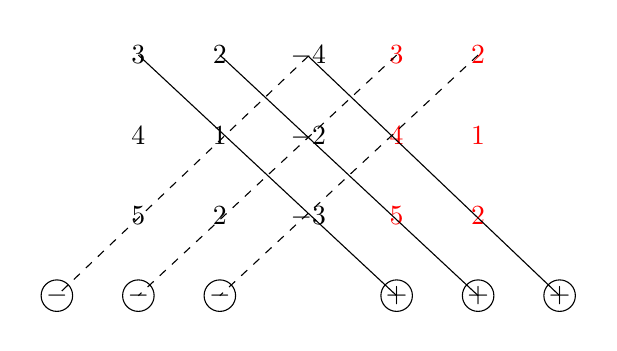
\begin{tikzpicture}               
    \matrix(A) [matrix of math nodes,nodes in empty cells,ampersand replacement=\&,row sep=15pt,column sep=15pt] {
      \&  3 \& 2 \& -4  \& \red{3} \& \red{2} \&\\
      \&  4 \& 1 \& -2  \& \red{4} \& \red{1} \&\\
      \&  5 \& 2 \& -3  \& \red{5} \& \red{2} \&\\
      -   \&    -        \&   -        \&               \&   +         \&   +        \& +\\
    };
    \draw[] (A-1-2.center) -- (A-4-5.center);
    \draw[] (A-1-3.center)  -- (A-4-6.center);
    \draw[] (A-1-4.center) -- (A-4-7.center); 
    \draw[dashed] (A-1-6.center) -- (A-4-3.center);
    \draw[dashed] (A-1-5.center) -- (A-4-2.center);
    \draw[dashed] (A-1-4.center) -- (A-4-1.center);
    \draw (A-4-1.center) circle (0.2cm);
    \draw (A-4-2.center) circle (0.2cm);
    \draw (A-4-3.center) circle (0.2cm);
    \draw (A-4-5.center) circle (0.2cm);
    \draw (A-4-6.center) circle (0.2cm);
    \draw (A-4-7.center) circle (0.2cm);

  \end{tikzpicture}               
\end{figure}

\begin{jie}
$$
\begin{array}{rl}
  \mbox{原式} &=
                3\cdot1\cdot(-3)+2\cdot(-2)\cdot5+(-4)\cdot4\cdot2-(-4)\cdot1\cdot5-3\cdot(-2)\cdot2-2\cdot4\cdot(-3)\\[0.2cm]
              &= -9-20-32+20+12+24 = -5.
\end{array}
$$    
\end{jie}



\begin{li}
  $$
  \left|
    \begin{array}{rrr}
      1&2&3\\
      4&5&6\\
      7&8&9
    \end{array}
  \right|
  $$
\end{li}

\begin{jie}
$$
\mbox{原式} \xlongequal[r_2-r_1]{r_3-r_2}  \left|
  \begin{array}{ccc}
    1&2&3\\
    3&3&3\\
    3&3&3
  \end{array}
\right|=0.
$$    
\end{jie}


\begin{li}
  $$
  \left|
    \begin{array}{rrr}
      2&2&1\\
      4&1&-1\\
      202&199&101
    \end{array}
  \right|
  $$
\end{li}

\begin{jie}
$$
\begin{array}{rl}
  \mbox{原式} & \xlongequal[]{c_1-c_2}  \left|
                \begin{array}{rrr}
                  0&2&1\\
                  3&1&-1\\
                  3&199&101
                \end{array}
                         \right| \xlongequal[]{r_3-r_2}  \left|
                         \begin{array}{rrr}
                           0&2&1\\
                           3&1&-1\\
                           0&198&102
                         \end{array}
                                  \right| \\[0.2in]
              & = (-1)^{2+1}\cdot 3 \cdot \left|
                \begin{array}{rr}
                  2&1\\
                  198&102
                \end{array}
                       \right| = -3 \cdot  (2\cdot 102-198)=-18.
\end{array}
$$
\end{jie}
    

\begin{li}
  $$
  \left|
    \begin{array}{ccc}
      1&\omega&\omega^2\\
      \omega^2&1&\omega\\
      \omega&\omega^2&1
    \end{array}
  \right|, \quad \omega = -\frac12 + i \frac{\sqrt{3}}2
  $$
\end{li}

\begin{jie}
 注意到$\omega^3=1$,故
$$
\omega \left|
  \begin{array}{ccc}
    1&\omega&\omega^2\\
    \omega^2&1&\omega\\
    \omega&\omega^2&1
  \end{array}
\right| = \left|
  \begin{array}{ccc}
    1&\omega&\omega^2\\
    \omega^3&\omega&\omega^2\\
    \omega&\omega^2&1
  \end{array}
\right| = \left|
  \begin{array}{ccc}
    1&\omega&\omega^2\\
    1&\omega&\omega^2\\
    \omega&\omega^2&1
  \end{array}
\right| = 0,
$$
从而
$$
\mbox{原式}=0.
$$
\end{jie}


\begin{li}
  $$
  \left|
    \begin{array}{ccc}
      1&x&x\\
      x&2&x\\
      x&x&3
    \end{array}
  \right|.
  $$
\end{li}

\begin{jie}
$$
\begin{array}{rl}
  \mbox{原式} & \xlongequal[r_3-xr_1]{r_2-xr_1} \left|
                \begin{array}{ccc}
                  1&x&x\\
                  0&2-x^2&x-x^2\\
                  0&x-x^2&3-x^2
                \end{array}
                           \right| = \left|
                           \begin{array}{cc}
                             2-x^2&x-x^2\\
                             x-x^2&3-x^2
                           \end{array}
                                    \right| \\[0.2in]
              &= (2-x^2)(3-x^2)-(x-x^2)^2=2x^3-6x^2+6.      
\end{array}
$$
\end{jie} 


\begin{li}
  $$
  \left|
    \begin{array}{cccc}
      0&0&0&4\\
      0&0&4&3\\
      0&4&3&2\\
      4&3&2&1\\
    \end{array}
  \right|
  $$
\end{li}

\begin{jie}
$$
\begin{array}{rl}
  \mbox{原式} & = (-1)^{1+4} \cdot 4 \cdot \left|
                \begin{array}{cccc}
                  0&0&\red{4}\\
                  0&4&3\\
                  4&3&2\\
                \end{array}
  \right| \\[0.2in]
              & = (-1)^{1+4} \cdot 4 \cdot (-1)^{1+3} \cdot 4 \cdot \left|
                \begin{array}{cccc}
                  0&4\\
                  4&3\\
                \end{array}
  \right| \\[0.2in]
              & = -4\cdot 4 \cdot (-16) = 256.
\end{array}
$$
\end{jie} 


\begin{li}
  $$
  \left|
    \begin{array}{cccccc}
      0&0&\cd&0&1&0\\
      0&0&\cd&2&0&0\\
      \vd&\vd&&\vd&\vd&\vd\\
      0&8&\cd&0&0&0\\
      9&0&\cd&0&0&0\\
      0&0&\cd&0&0&10\\
    \end{array}
  \right|
  $$
\end{li}

\begin{jie}
$$
\begin{array}{rl}
  \mbox{原式} & = (-1)^{10+10} \cdot 10 \cdot \left|
                \begin{array}{cccccc}
                  0&0&\cd&0&1\\
                  0&0&\cd&2&0\\
                  \vd&\vd&&\vd&\vd\\
                  0&8&\cd&0&0\\
                  9&0&\cd&0&0\\
                \end{array}
  \right| = 10 \cdot (-1)^{\frac{9\times 8}2} 9! = 10!
\end{array}
$$
\end{jie} 



\begin{li}
  $$
  \left|
    \begin{array}{rrrr}
      1&1&1&1\\
      1&-1&1&1\\
      1&1&-1&1\\
      1&1&1&-1\\
    \end{array}
  \right|
  $$
\end{li}

\begin{jie}
$$
\mbox{原式}  \xlongequal[i=2,3,4]{r_i-r_1} \left|
  \begin{array}{rrrr}
    1&1&1&1\\
    0&-2&0&0\\
    0&0&-2&0\\
    0&0&0&-2
  \end{array}
\right|  = (-2)^3 = -8.
$$
\end{jie}


\begin{li}
  $$
  \left|
    \begin{array}{rrrr}
      1&2&3&4\\
      2&3&4&1\\
      3&4&1&2\\
      4&1&2&3\\
    \end{array}
  \right|
  $$
\end{li}

\begin{jie}

$$
\begin{array}{rl}
  \mbox{原式}  & \xlongequal[i=4,3,2]{r_i-r_{i-1}} \left|
                 \begin{array}{rrrr}
                   1&2&3&4\\
                   1&1&1&-3\\
                   1&1&-3&1\\
                   1&-3&1&1\\
                 \end{array}
  \right| 
  \xlongequal[i=2,3,4]{c_i-c_1}  \left|
  \begin{array}{rrrr}
    1&1&2&3\\
    1&0&0&-4\\
    1&0&-4&0\\
    1&-4&0&0\\
  \end{array}
  \right| \\[0.25in] 
               &  \xlongequal[i=2,3,4]{c_i\div 4} 4^3 \left|
                 \begin{array}{rrrr}
                   1&\frac14&\frac24&\frac34\\
                   1&0&0&-1\\
                   1&0&-1&0\\
                   1&-1&0&0\\
                 \end{array}
  \right| 
  \xlongequal[]{c_1+c_2+c_3+c_4} 4^3 \left|
  \begin{array}{rrrr}
    1+\frac{1+2+3}4&\frac14&\frac24&\frac34\\
    0&0&0&-1\\
    0&0&-1&0\\
    0&-1&0&0\\
  \end{array}
  \right| \\[0.25in] 
               &  \ds =4^3 \frac{10}4 \left|
                 \begin{array}{rrrr}
                   0&0&-1\\
                   0&-1&0\\
                   -1&0&0\\
                 \end{array}
  \right| = 160.
\end{array}
$$

\end{jie}



\begin{li}
  $$
  \left|
    \begin{array}{rrrr}
      5&0&4&2\\
      1&-1&2&1\\
      4&1&2&0\\
      1&1&1&1\\
    \end{array}
  \right|
  $$
\end{li}

\begin{jie}

$$
\begin{array}{rl}
  \mbox{原式}  & \xlongequal[r_4+r_2]{r_3+r_2}
                 \left|
                 \begin{array}{rrrr}
                   5&0&4&2\\
                   1&\red{-1}&2&1\\
                   5&0&4&1\\
                   2&0&3&2\\
                 \end{array}
  \right|  = (-1)^{2+2}\cdot (-1)\cdot       \left|
  \begin{array}{rrr}
    5&4&2\\
    5&4&1\\
    2&3&2\\
  \end{array}
  \right| \\[0.25in]
               &  \xlongequal[]{r_1-r_2}
                 -\left|
                 \begin{array}{rrr}
                   0&0&\red{1}\\
                   5&4&1\\
                   2&3&2\\
                 \end{array}
  \right| 
  = - (-1)^{1+3} \cdot 1 \cdot \left|
  \begin{array}{rrr}
    5&4\\
    2&3
  \end{array}
       \right| = -7.
\end{array}
$$
\end{jie}



\begin{li}
  $$
  \left|
    \begin{array}{rrrrr}
      3&6&5&6&4\\
      2&5&4&5&3\\
      3&6&3&4&2\\
      2&5&4&6&5\\
      1&1&1&-1&-1
    \end{array}
  \right|
  $$
\end{li}

\begin{jie}
$$
\begin{array}{rl}
  \mbox{原式}  &  \xlongequal[]{r_2 \leftrightarrow r_3}
                 -\left|
                 \begin{array}{rrrrr}
                   3&6&5&6&4\\
                   3&6&3&4&2\\
                   2&5&4&5&3\\
                   2&5&4&6&5\\
                   1&1&1&-1&-1
                 \end{array}
                             \right| 
                             \xlongequal[r_1-r_3]{r_2-r_1 \atop r_4-r_3} -\left|
                             \begin{array}{rrrrr}
                               1&1&1&1&1\\
                               0&0&-2&-2&-2\\
                               2&5&4&5&3\\
                               0&0&0&1&2\\
                               1&1&1&-1&-1
                             \end{array}
                                         \right| \\[0.4in]
               &  \xlongequal[r_5-r_1]{r_3-2r_1}  -\left|
                 \begin{array}{rrrrr}
                   1&1&1&1&1\\
                   0&0&-2&-2&-2\\
                   0&3&2&3&1\\
                   0&0&0&1&2\\
                   0&0&0&-2&-2
                 \end{array}
                             \right| 
                             \xlongequal[r_5+2r_4]{r_2\leftrightarrow r_3}  \left|
                             \begin{array}{rrrrr}
                               1&1&1&1&1\\
                               0&3&2&3&1\\
                               0&0&-2&-2&-2\\
                               0&0&0&1&2\\
                               0&0&0&0&2
                             \end{array}
                                        \right|\\[0.4in]
               &  = -12.
\end{array}
$$
\end{jie} 


\begin{li}
  $$
  \left|
    \begin{array}{rrrr}
      1&2&0&0\\
      3&4&0&0\\
      0&0&-1&3\\
      0&0&5&1\\
    \end{array}
  \right|
  $$
\end{li}

\begin{jie}

$$
\mbox{原式} = \left|
  \begin{array}{cc}
    1&2\\
    3&4      
  \end{array}
\right| \cdot
\left|
  \begin{array}{rr}
    -1&3\\
    5&1      
  \end{array}
\right| = (-2)\cdot(-16)=32.
$$
\end{jie}


\begin{li}
  $$
  \left|
    \begin{array}{rrrrr}
      1&2&3&4&5\\
      6&7&8&9&10\\
      0&0&0&1&3\\
      0&0&0&2&4\\
      0&1&0&1&1
    \end{array}
  \right|
  $$
\end{li}

 
$$
\begin{array}{rl}
  \mbox{原式} &  \ds \xlongequal[]{r_3\leftrightarrow r_5}
                -\left|
                \begin{array}{rrrrr}
                  \red{1}&\red{2}&\red{3}&4&5\\
                  \red{6}&\red{7}&\red{8}&9&10\\
                  \red{0}&\red{1}&\red{0}&1&1\\
                  0&0&0&\blue{2}&\blue{4}\\
                  0&0&0&\blue{1}&\blue{3}
                \end{array}
                                  \right|  = -\left|
                                  \begin{array}{rrr}
                                    1&2&3\\
                                    6&7&8\\
                                    0&\red{1}&0\\
                                  \end{array}
  \right| \cdot \left|
  \begin{array}{rr}
    2&4\\
    1&3\\
  \end{array}
  \right|\\[0.4in]
              & =-(-1)^{3+2} \cdot 1 \cdot \left|
                \begin{array}{rrr}
                  1&3\\
                  6&8
                \end{array}
                     \right| \cdot \left|
                     \begin{array}{rr}
                       2&4\\
                       1&3\\
                     \end{array}
  \right| \\[0.2in]
              & =   (-10) \cdot 2 = -20.
\end{array}
$$





\begin{li}
  $$
  \left|
    \begin{array}{rrrrr}
      0&0&1&-1&2\\
      0&0&3&0&2\\
      0&0&2&4&0\\
      1&2&4&0&-1\\
      3&1&2&5&8
    \end{array}
  \right|
  $$
\end{li}

\begin{jie}
$$
\begin{array}{rl}
  \mbox{原式} &
                \xlongequal[c_2\leftrightarrow c_1]{c_3\leftrightarrow c_2}
                \left|
                \begin{array}{rrrrr}
                  1&0&0&-1&2\\
                  3&0&0&0&2\\
                  2&0&0&4&0\\
                  4&1&2&0&-1\\
                  2&3&1&5&8
                \end{array}
                           \right|
                           
                           \xlongequal[c_3\leftrightarrow c_2]{c_4\leftrightarrow c_3}
                           \left|
                           \begin{array}{rrrrr}
                             1&-1&0&0&2\\
                             3&0&0&0&2\\
                             2&4&0&0&0\\
                             4&0&1&2&-1\\
                             2&5&3&1&8
                           \end{array}
                                      \right| \\[0.35in]
              &  \xlongequal[c_4\leftrightarrow c_3]{c_5\leftrightarrow c_4}
                \left|
                \begin{array}{rrrrr}
                  1&-1& 2&0&0\\
                  3& 0& 2&0&0\\
                  2& 4& 0&0&0\\
                  4& 0&-1&1&2\\
                  2& 5& 8&3&1
                \end{array}
                             \right|  = \left|
                             \begin{array}{rrrrr}
                               1&-1& 2\\
                               3& 0& 2\\
                               2& 4& 0
                             \end{array}
                                     \right|\cdot \left|
                                     \begin{array}{rr}
                                       1&2\\
                                       3&1
                                     \end{array}
                                          \right| \\[0.35in]
              &  \xlongequal[]{r_2-r_1} \left|
                \begin{array}{rrrrr}
                  1&-1& 2\\
                  2& 1& 0\\
                  2& 4& 0
                \end{array}
                        \right| \left|
                        \begin{array}{rr}
                          1&2\\
                          3&1
                        \end{array}
                             \right| =   2  \left|
                             \begin{array}{rrrrr}
                               2& 1\\
                               2& 4
                             \end{array}
                                  \right| \left|
                                  \begin{array}{rr}
                                    1&2\\
                                    3&1
                                  \end{array}
                                       \right|  = 2 \cdot 6 \cdot (-5) = -60.
\end{array}
$$
\end{jie} 


\begin{li}
  $$
  \left|
    \begin{array}{cc}
      *&\A\\
      \B&\zero
    \end{array}
  \right|, \quad
  \A = \left|
    \begin{array}{ccc}
      1&0&0\\
      1&2&0\\
      1&2&3
    \end{array}
  \right|, \quad
  \B = \left|
    \begin{array}{rrrrr}
      &&&&-1\\
      &&&-2&\\
      &&-3&&\\
      &-4&&&\\
      -5&&&&
    \end{array}
  \right|
  $$
\end{li}

\begin{jie}
$$
\begin{array}{rl}
  \mbox{原式} &= (-1)^{3\times 5}  \left|
                \begin{array}{rr}
                  \A&*\\
                  \zero&\B
                \end{array}
                         \right| \\[0.2in]
              & = (-1) \cdot  |\A|\cdot |\B| \\[0.1in]
              &= (-1) \cdot 1\cdot 2\cdot 3 \cdot (-1)^{\frac{5\times 4}2} (-1)(-2)(-3)(-4)(-5)\\[0.1in]
              &= 6\times 120 =720
\end{array}
$$
\end{jie}


\begin{li}
  证明:
  $$
  \left|
    \begin{array}{ccc}
      a_1+b_1x & a_1x+b_1 & c_1\\
      a_2+b_2x & a_2x+b_2 & c_2\\
      a_3+b_3x & a_3x+b_3 & c_3        
    \end{array}
  \right| = (1-x^2) \left|
    \begin{array}{ccc}
      a_1&b_1&c_1\\
      a_2&b_2&c_2\\
      a_3&b_3&c_3
    \end{array}
  \right|
  $$
\end{li}

\begin{proof}
$$
\begin{array}{rl}
  \mbox{左边} &= \left|
                \begin{array}{ccc}
                  a_1 & a_1x+b_1 & c_1\\
                  a_2 & a_2x+b_2 & c_2\\
                  a_3 & a_3x+b_3 & c_3        
                \end{array}
                                   \right| + \left|
                                   \begin{array}{ccc}
                                     b_1x & a_1x+b_1 & c_1\\
                                     b_2x & a_2x+b_2 & c_2\\
                                     b_3x & a_3x+b_3 & c_3        
                                   \end{array}
                                                       \right|\\[0.2in]
              &= \left|
                \begin{array}{ccc}
                  a_1 & a_1x+b_1 & c_1\\
                  a_2 & a_2x+b_2 & c_2\\
                  a_3 & a_3x+b_3 & c_3        
                \end{array}
                                   \right| + x\left|
                                   \begin{array}{ccc}
                                     b_1 & a_1x+b_1 & c_1\\
                                     b_2 & a_2x+b_2 & c_2\\
                                     b_3 & a_3x+b_3 & c_3        
                                   \end{array}
                                                      \right|\\[0.2in]
              &= \left|
                \begin{array}{ccc}
                  a_1 & a_1x & c_1\\
                  a_2 & a_2x & c_2\\
                  a_3 & a_3x & c_3        
                \end{array}
                               \right| + \left|
                               \begin{array}{ccc}
                                 a_1 & b_1 & c_1\\
                                 a_2 & b_2 & c_2\\
                                 a_3 & b_3 & c_3        
                               \end{array}
                                             \right| +  x\left|
                                             \begin{array}{ccc}
                                               b_1 & a_1x & c_1\\
                                               b_2 & a_2x & c_2\\
                                               b_3 & a_3x & c_3        
                                             \end{array}
                                                            \right| +  x\left|
                                                            \begin{array}{ccc}
                                                              b_1 & b_1 & c_1\\
                                                              b_2 & b_2 & c_2\\
                                                              b_3 & b_3 & c_3        
                                                            \end{array}
                                                                          \right|\\[0.2in]
              &=  \left|
                \begin{array}{ccc}
                  a_1 & b_1 & c_1\\
                  a_2 & b_2 & c_2\\
                  a_3 & b_3 & c_3        
                \end{array}
                              \right| +  x\left|
                              \begin{array}{ccc}
                                b_1 & a_1x & c_1\\
                                b_2 & a_2x & c_2\\
                                b_3 & a_3x & c_3        
                              \end{array}
                                             \right|  = (1-x^2)\left|
                                             \begin{array}{ccc}
                                               a_1 & b_1 & c_1\\
                                               a_2 & b_2 & c_2\\
                                               a_3 & b_3 & c_3        
                                             \end{array}
                                                           \right| = \mbox{右边}
\end{array}
$$
\end{proof}





\begin{li}
  证明:
  $$
  \left|
    \begin{array}{cccc}
      1+x&1&1&1\\
      1&1-x&1&1\\
      1&1&1+y&1\\
      1&1&1&1-y
    \end{array}
  \right|=x^2y^2.
  $$
\end{li}

\begin{proof}
$$
\begin{array}{rl}
  \mbox{左边} &  = \left|
                \begin{array}{ccccc}
                  \red{1}&\red{1}&\red{1}&\red{1}&\red{1}\\
                  \red{0}&1+x&1&1&1\\
                  \red{0}&1&1-x&1&1\\
                  \red{0}&1&1&1+y&1\\
                  \red{0}&1&1&1&1-y
                \end{array}
                                 \right| \\[0.4in]
              & \xlongequal[i=2,3,4,5]{r_i-r_1} \left|
                \begin{array}{ccccc}
                  \red{1}&\red{1}&\red{1}&\red{1}&\red{1}\\
                  \red{-1}&x&0&0&0\\
                  \red{-1}&0&-x&0&0\\
                  \red{-1}&0&0&y&0\\
                  \red{-1}&0&0&0&-y
                \end{array}
                                  \right|
                                  
                                  \xlongequal[c_1+ c_4/y \atop c_1 -c_5/y ]{c_1+ c_2/x \atop c_1 -c_3/x } \left|
                                  \begin{array}{ccccc}
                                    \red{1}&\red{1}&\red{1}&\red{1}&\red{1}\\
                                    \red{0}&x&0&0&0\\
                                    \red{0}&0&-x&0&0\\
                                    \red{0}&0&0&y&0\\
                                    \red{0}&0&0&0&-y
                                  \end{array}
                                                   \right| \\[0.4in]
              & = x^2y^2.
\end{array}
$$
\end{proof}




\begin{li}
  证明:
  $$
  \left|
    \begin{array}{ccc}
      1   &   1   &   1\\
      a   &   b   &   c\\
      a^3 &   b^3 &   c^3
    \end{array}
  \right| = (a-b)(a-c)(b-c)(a+b+c).
  $$
\end{li}

\begin{proof}
考察范德蒙德行列式
$$
\left|
  \begin{array}{cccc}
    1   &   1   &   1   & \red{1}\\
    a   &   b   &   c   & \red{y}\\
    \red{a^2} &   \red{b^2} &   \red{c^2} & \purple{y^2}\\
    a^3 &   b^3 &   c^3 & \red{y^3}\\
  \end{array}
\right|
= (y-a)(y-b)(y-c)(c-a)(c-b)(b-a)
$$

等式两端均为关于$y$的多项式,比较$y^2$的系数,可知
$$
\left|
  \begin{array}{cccc}
    1   &   1   &   1  \\ 
    a   &   b   &   c  \\
    a^3 &   b^3 &   c^3\\
  \end{array}
\right| = (a-b)(a-c)(b-c)(a+b+c)
$$
\end{proof}






\begin{li}
  证明:
  $$
  \left|
    \begin{array}{ccc}
      1&a^2&a^3\\
      1&b^2&b^3\\
      1&c^2&c^3
    \end{array}
  \right| = (ab+bc+ca)\left|
    \begin{array}{ccc}
      1&a&a^2\\
      1&b&b^2\\
      1&c&c^2
    \end{array}
  \right|
  $$
\end{li}

\begin{proof}
考察范德蒙德行列式
$$
\left|
  \begin{array}{cccc}      
    1&\red{a}&a^2&a^3\\
    1&\red{b}&b^2&b^3\\
    1&\red{c}&c^2&c^3\\
    \red{1}&\purple{y}&\red{y^2}&\red{y^3}
  \end{array}
\right|
= (y-a)(y-b)(y-c)(c-a)(c-b)(b-a)
$$

等式两端均为关于$y$的多项式,比较$y$的系数,可知
$$
\left|
  \begin{array}{cccc}
    1   &   1   &   1  \\ 
    a^2 &   b^2 &   c^2  \\
    a^3 &   b^3 &   c^3\\
  \end{array}
\right| = (a-b)(a-c)(b-c)(ab+bc+ca) = (ab+bc+ca)\left|
  \begin{array}{ccc}
    1&a&a^2\\
    1&b&b^2\\
    1&c&c^2
  \end{array}
\right|
$$

\end{proof}

\begin{li}
  计算
  $$
  \left|
    \begin{array}{cccc}
      1&0&2&a\\
      2&0&b&0\\
      3&c&4&5\\
      d&0&0&0
    \end{array}
  \right|
  $$
\end{li}

\begin{jie}
$$
\begin{array}{rl}
  \mbox{左边} &  \xlongequal[]{\mbox{按第4行展开}}
                (-1)^{4+1} \cdot d \cdot \left|
                \begin{array}{ccc}
                  0&2&a\\
                  0&b&0\\
                  c&4&5
                \end{array}
                       \right| \\[0.4in]
              &  \xlongequal[]{\mbox{按第2行展开}}
                (-d) \cdot (-1)^{2+2} \cdot b \left|
                \begin{array}{ccc}
                  0&a\\
                  c&5
                \end{array}
                     \right| = abcd.
\end{array}
$$
\end{jie}

\begin{li}
  计算
  $$
  \left|
    \begin{array}{ccccc}
      a&1&0&0\\
      -1&b&1&0\\
      0&-1&c&1\\
      0&0&-1&d
    \end{array}
  \right|
  $$
\end{li}

\begin{jie}
$$
\begin{array}{rl}
  \mbox{左边} &  \xlongequal[]{\mbox{按第1行展开}}
                (-1)^{1+1} \cdot a \cdot \left|
                \begin{array}{ccc}        
                  b&1&0\\
                  -1&c&1\\
                  0&-1&d
                \end{array}
                        \right| + (-1)^{1+2} \cdot 1 \cdot\left|
                        \begin{array}{ccccc}
                          -1&1&0\\
                          0&c&1\\
                          0&-1&d
                        \end{array}
                                \right|
  \\[0.4in]
              &  = a \cdot \left|
                \begin{array}{ccc}        
                  b&1&0\\
                  -1&c&1\\
                  0&-1&d
                \end{array}
                        \right| +\left|
                        \begin{array}{ccccc}
                          c&1\\
                          -1&d
                        \end{array}
                              \right|\\[0.4in]
              &  \xlongequal[]{\mbox{按第1行展开}}
                a \cdot \left( b \cdot \left|
                \begin{array}{ccc}
                  c&1\\
                  -1&d
                \end{array}
                      \right| + (-1)^{1+2}\cdot 1 \cdot \left|
                      \begin{array}{cc}
                        -1&1\\
                        0& d
                      \end{array}
                           \right| \right) + (cd+1)\\[0.2in]
              & = a(b(cd+1)+d)+(cd+1) = (ab+1)(cd+1)+ad
\end{array}
$$
\end{jie}


\begin{li}
  计算
  $$
  \left|
    \begin{array}{cccc}
      a^2&(a+1)^2&(a+2)^2&(a+3)^2\\[0.1cm]
      b^2&(b+1)^2&(b+2)^2&(b+3)^2\\[0.1cm]
      c^2&(c+1)^2&(c+2)^2&(c+3)^2\\[0.1cm]
      d^2&(d+1)^2&(d+2)^2&(d+3)^2
    \end{array}
  \right|
  $$
\end{li}

\begin{jie}
$$
\begin{array}{rl}
  \mbox{左边} &  \xlongequal[c_2-c_1]{c_4-c_3\atop c_3-c_2}
                \left|
                \begin{array}{cccc}
                  a^2&2a+1&2a+3&2a+5\\[0.1cm]
                  b^2&2b+1&2b+3&2b+5\\[0.1cm]
                  c^2&2c+1&2c+3&2c+5\\[0.1cm]
                  d^2&2d+1&2d+3&2d+5
                \end{array}
                                 \right|\\[0.4in]
              & \xlongequal[c_3-c_2]{c_4-c_3}
                \left|
                \begin{array}{cccc}
                  a^2&2a+1&2&2\\[0.1cm]
                  b^2&2b+1&2&2\\[0.1cm]
                  c^2&2c+1&2&2\\[0.1cm]
                  d^2&2d+1&2&2
                \end{array}
                              \right| = 0.
\end{array}
$$
\end{jie}


\begin{li}
  计算
  $$
  \left|
    \begin{array}{cccc}
      a&b&c&1\\
      b&c&a&1\\
      c&a&b&1\\
      \frac{b+c}2&\frac{c+a}2&\frac{a+b}2&1        
    \end{array}
  \right|
  $$
\end{li}

\begin{jie}
$$
\mbox{原式}  \xlongequal[]{r_3+r_1+r_2}
\left|
  \begin{array}{cccc}
    a&b&a+b+c&1\\
    b&c&a+b+c&1\\
    c&a&a+b+c&1\\
    \frac{b+c}2&\frac{c+a}2&a+b+c&1
  \end{array}
\right| = 0 .
$$
\end{jie}



\begin{li}
  计算
  $$
  \left|
    \begin{array}{cccc}
      a_1&0&0&b_1\\
      0&a_2&b_2&0\\
      0&b_3&a_3&0\\
      b_4&0&0&a_4
    \end{array}
  \right|
  $$
\end{li}

\begin{jie}
$$
\begin{array}{rl}
  \mbox{原式} &\xlongequal[c_3\leftrightarrow c_2]{c_4\leftrightarrow c_3}
                \left|
                \begin{array}{cccc}
                  a_1&b_1&0  &  0\\
                  0  &0  &a_2&b_2\\
                  0  &0  &b_3&a_3\\
                  b_4&a_4&0  &  0
                \end{array}
                               \right|\\[0.4in]
              & \xlongequal[r_3\leftrightarrow r_2]{r_4\leftrightarrow r_3}
                \left|
                \begin{array}{cccc}
                  a_1&b_1&0  &  0\\
                  b_4&a_4&0  &  0\\
                  0  &0  &a_2&b_2\\
                  0  &0  &b_3&a_3      
                \end{array}
                               \right|
                               = (a_1a_4-b_1b_4)(a_2a_3-b_2b_3) .
                               
\end{array}
$$
\end{jie}


\begin{li}
  计算
  $$
  \left|
    \begin{array}{cccccc}
      1&2&2&\cd&2&2\\
      2&2&2&\cd&2&2\\
      2&2&3&\cd&2&2\\
      \vd&\vd&\vd&\dd&\vd&\vd\\
      2&2&2&\cd&n-1&2\\
      2&2&2&\cd&2&n        
    \end{array}
  \right|
  $$
\end{li}

\begin{jie}
$$
\begin{array}{rl}
  \mbox{原式} & = \left|
                \begin{array}{ccccccc}
                  1&2&2&2&\cd&2&2\\
                  0&1&2&2&\cd&2&2\\
                  0&2&2&2&\cd&2&2\\
                  0&2&2&3&\cd&2&2\\
                  \vd&\vd&\vd&\vd&\dd&\vd&\vd\\
                  0&2&2&2&\cd&n-1&2\\
                  0&2&2&2&\cd&2&n        
                \end{array}
                                 \right|  = \left|
                \begin{array}{ccccccc}
                  1&2&2&2&\cd&2&2\\
                  -1&-1&0&0&\cd&0&0\\
                  \red{-1}&0&0&0&\cd&0&0\\
                  -1&0&0&1&\cd&0&0\\
                  \vd&\vd&\vd&\vd&\dd&\vd&\vd\\
                  -1&0&0&0&\cd&n-3&0\\
                  -1&0&0&0&\cd&0&n-2        
                \end{array}
                                  \right| \\[0.6in]
              & =(-1)^{3+1} (-1)\left|
                \begin{array}{ccccccc}
                  2&2&2&\cd&2&2\\
                  -1&0&0&\cd&0&0\\
                  0&0&1&\cd&0&0\\
                  \vd&\vd&\vd&\dd&\vd&\vd\\
                  0&0&0&\cd&n-3&0\\
                  0&0&0&\cd&0&n-2        
                \end{array}
                               \right|
  \\[0.2in]
              & = -2 (n-2)!
\end{array}
$$    

\end{jie}


\begin{li}
  计算
  $$
  \left|
    \begin{array}{ccccc}
      1&1&1&\cd&1\\[0.1cm]
      a&a-1&a-2&\cd&a-n\\[0.1cm]
      a^2&(a-1)^2&(a-2)^2&\cd&(a-n)^2\\[0.1cm]
      \vd&\vd&\vd&&\vd\\[0.1cm]
      a^n&(a-1)^n&(a-2)^n&\cd&(a-n)^n      
    \end{array}
  \right|
  $$      
\end{li}

\begin{jie}
该行列式为范德蒙行列式, 故
$$
\begin{array}{rl}
  \mbox{原式} & = \prod_{n\ge i > j \ge 0} [(a-i)-(a-j)] \\[0.4cm]
              &= \prod_{n\ge i > j \ge 0} (j-i) \\[0.4cm]
              & = (-1)^{\frac{n(n+1)}2} \prod_{n\ge i > j \ge 0} (i-j) \\[0.4cm]
              & = (-1)^{\frac{n(n+1)}2} \prod_{i=1}^n i!      
\end{array}
$$
\end{jie}


\begin{li}
  计算
  $$
  \left|
    \begin{array}{cccccc}
      a_1^n&a_1^{n-1}b_1&a_1^{n-2}b_1^2&\cd&a_1b_1^{n-1}&b_1^n\\[0.1cm]
      a_2^n&a_2^{n-1}b_2&a_2^{n-2}b_2^2&\cd&a_2b_2^{n-1}&b_2^n\\[0.1cm]
      \vd&\vd&\vd&&\vd&\vd\\[0.1cm]
      a_{n+1}^n&a_{n+1}^{n-1}b_{n+1}&a_{n+1}^{n-2}b_{n+1}^2&\cd&a_{n+1}b_{n+1}^{n-1}&b_{n+1}^n\\[0.1cm]
    \end{array}
  \right|
  $$
\end{li}

\begin{jie}
$$
\begin{array}{rl}
  \mbox{原式} &  = a_1^n a_2^n \cd a_{n+1}^n \left|
                \begin{array}{cccccc}
                  1&a_1^{-1}b_1&(a_1^{-1}b_1)^2&\cd&(a_1^{-1}b_1)^{n-1}&(a_1^{-1}b_1)^n\\[0.1cm]
                  1&a_2^{-1}b_2&(a_2^{-1}b_2)^2&\cd&(a_2^{-1}b_2)^{n-1}&(a_2^{-1}b_2)^n\\[0.1cm]
                  \vd&\vd&\vd&&\vd&\vd\\[0.1cm]
                  1&a_{n+1}^{-1}b_{n+1}&(a_{n+1}^{-1}b_{n+1})^2&\cd&(a_{n+1}^{-1}b_{n+1})^{n-1}&(a_{n+1}^{-1}b_{n+1})^n\\[0.1cm]
                \end{array}
  \right| \\[0.4in]
              &  \ds = a_1^n a_2^n \cd a_{n+1}^n \prod_{n+1\ge i > j \ge 1} \left(\frac{b_i}{a_i}-\frac{b_j}{a_j}\right)
  \\[0.2in]
              &  \ds =   \prod_{n+1\ge i > j \ge 1} (b_ia_j-a_ib_j)
\end{array}
$$
\end{jie}





\begin{li}
  用克拉默法则求
  $$
  \left\{
    \begin{array}{rcrcrcrcrc}
      5x_1&&&+&4x_3&+&2x_4&=&3,\\[0.1cm]
      x_1&-&x_2&+&2x_3&+& x_4&=&1,\\[0.1cm]
      4x_1&+&x_2&+&2x_3& & &=&1,\\[0.1cm]
      x_1&+&x_2&+& x_3&+&x_4&=&0.
    \end{array}
  \right.
  $$
\end{li}

\begin{jie}
$$
\begin{array}{rl}
  D & = \left|
      \begin{array}{rrrr}
        5&0&4&2\\
        1&-1&2&1\\
        4&1&2&0\\
        1&1&1&1
      \end{array}
               \right| = -7, \\[0.3in]  
  D_1 & = \left|
        \begin{array}{rrrr}
          \red{3}&0&4&2\\
          \red{1}&-1&2&1\\
          \red{1}&1&2&0\\
          \red{0}&1&1&1
        \end{array}
                       \right| \xlongequal[r_4+r_2]{r_3+r_2} \left|
                       \begin{array}{rrrr}
                         3&0&4&2\\
                         1&-1&2&1\\
                         2&0&4&1\\
                         1&0&3&2
                       \end{array}
                                \right| =  (-1)^{2+2} (-1) \left|
                                \begin{array}{rrrr}
                                  3&4&2\\
                                  2&4&1\\
                                  1&3&2
                                \end{array}
                                       \right| \\[0.3in]
    & \xlongequal[r_3-2r_2]{r_1-2r_2}  - \left|
      \begin{array}{rrrr}
        -1&-4&0\\
        2&4&1\\
        -3&-5&0
      \end{array}
               \right|  = - (-1)^{2+3} \cdot  \left|
               \begin{array}{rrrr}
                 -1&-4\\
                 -3&-5
               \end{array}
                     \right| = -7,
\end{array}
$$





$$
\begin{array}{rl}
  D_2 &=\left|
        \begin{array}{rrrr}
          5&\red{3}&4&2\\
          1&\red{1}&2&1\\
          4&\red{1}&2&0\\
          1&\red{0}&1&1
        \end{array}
                       \right| 
                       \xlongequal[c_4-c_1]{c_3-c_1}
                       \left|
                       \begin{array}{rrrr}
                         5&\red{3}&-1&-3\\
                         1&\red{1}& 1& 0\\
                         4&\red{1}&-2&-4\\
                         1&\red{0}& 0& 0
                       \end{array}
                                       \right|
                                       
                                       =  (-1)^{4+1} \cdot 
                                       \left|
                                       \begin{array}{rrrr}
                                         3&-1&-3\\
                                         1& 1& 0\\
                                         1&-2&-4\\       
                                       \end{array}
  \right|  \\[0.3in]
      & \xlongequal[]{c_1-c_2}
        -\left|
        \begin{array}{rrrr}
          4&-1&-3\\
          0& 1& 0\\
          3&-2&-4\\       
        \end{array}
  \right|  = -(-1)^{2+2} \cdot \left|
  \begin{array}{rrrr}
    4&-3\\
    3&-4\\       
  \end{array}
  \right| = 7,   \\[0.4in]   
  D_3 &  = \left|
        \begin{array}{rrrr}
          5& 0&\red{3}&2\\
          1&-1&\red{1}&1\\
          4& 1&\red{1}&0\\
          1& 1&\red{0}&1
        \end{array}
                        \right| 
                        \xlongequal[r_4+r_2]{r_3+r_2}
                        \left|
                        \begin{array}{rrrr}
                          5& 0&3&2\\
                          1&-1&1&1\\
                          5& 0&2&1\\
                          2& 0&1&2
                        \end{array}
                                  \right|
                                  
                                  =  (-1)^{2+2}  (-1)   
                                  \left|
                                  \begin{array}{rrrr}
                                    5&3&2\\
                                    5&2&1\\
                                    2&1&2
                                  \end{array}
                                         \right|  \\[0.3in]
      & \xlongequal[c_3-2c_2]{c_1-2c_2}
        -\left|
        \begin{array}{rrrr}
          -1&3&-4\\
          1&2&-3\\
          0&1& 0
        \end{array}
               \right|  = -(-1)^{3+2} \cdot \left|
               \begin{array}{rrrr}
                 -1&-4\\
                 1&-3\\       
               \end{array}
  \right| = 7
\end{array} 
$$






$$
\begin{array}{rl}
  D_4 &= \left|
        \begin{array}{rrrr}
          5&0&4&\red{3}\\
          1&-1&2&\red{1}\\
          4&1&2&\red{1}\\
          1&1&1&\red{0}\\
        \end{array}
  \right|
  
  \xlongequal[r_4+r_2]{r_3+r_2}
  \left|
  \begin{array}{rrrrr}
    5&0&4&{3}\\
    1&-1&2&{1}\\
    5&0&4&{2}\\
    2&0&3&{1}\\
  \end{array}
  \right| \\[0.4in]
      & =  -   
        \left|
        \begin{array}{rrr}
          5&4&{3}\\
          5&4&{2}\\
          2&3&{1}\\
        \end{array}
  \right| 
  \xlongequal[]{r_1-r_2}
  -\left|
  \begin{array}{rrr}
    0&0&{1}\\
    5&4&{2}\\
    2&3&{1}\\
  \end{array}\right| 
  =
  -\left|
  \begin{array}{rrr}
    5&4\\
    2&3\\
  \end{array}\right|
  = -7.
\end{array}
$$ 
由克拉默法则可知,
$$
\begin{array}{lll}
  \ds x_1 = \frac{D_1}D = 1, &
                               \ds x_2 = \frac{D_2}D = -1, \\[0.2in]
  \ds x_3 = \frac{D_3}D = -1, &
                                \ds x_4 = \frac{D_4}D = 1.
\end{array}
$$
\end{jie}


\begin{li}
  用克拉默法则求
  $$
  \left\{
    \begin{array}{rcrcrcrcrcrc}
      &&x_2&+&x_3&+&x_4&+&x_5=&1,\\[0.1cm]
      x_1&&&+&x_3&+&x_4&+&x_5&=&2,\\[0.1cm]
      x_1&+&x_2&&&+&x_4&+&x_5&=&3,\\[0.1cm]
      x_1&+&x_2&+&x_3& & &+&x_5&=&4,\\[0.1cm]
      x_1&+&x_2&+& x_3&+&x_4&&&=&5.
    \end{array}
  \right.
  $$
\end{li}

\begin{jie}
$$
\begin{array}{rl}
  D &= \left|
      \begin{array}{rrrrr}
        0&1&1&1&1\\
        1&0&1&1&1\\
        1&1&0&1&1\\
        1&1&1&0&1\\
        1&1&1&1&0\\
      \end{array}
  \right|
  \xlongequal[r_1\div 4]{r_1+r_2+\cd+r_5}
  4 \left|
  \begin{array}{rrrrr}
    1&1&1&1&1\\
    1&0&1&1&1\\
    1&1&0&1&1\\
    1&1&1&0&1\\
    1&1&1&1&0\\
  \end{array}
  \right| , \\[0.3in]
    & \xlongequal[i=2,\cd, 4]{r_i-r_1}
      4 \left|
      \begin{array}{rrrrr}
        1&1&1&1&1\\
        0&-1&0&0&0\\
        0&0&-1&0&0\\
        0&0&0&-1&0\\
        0&0&0&0&-1\\
      \end{array}
  \right| = 4.
\end{array}
$$







$$
\begin{array}{rl}
  D_1 &= \left|
        \begin{array}{rrrrr}
          \red{1}&1&1&1&1\\
          \red{2}&0&1&1&1\\
          \red{3}&1&0&1&1\\
          \red{4}&1&1&0&1\\
          \red{5}&1&1&1&0\\
        \end{array}
  \right| 
  \xlongequal[r_5-r_1]{r_3-r_1\atop r_4-r_1}
  \left|
  \begin{array}{rrrrr}
    {1}&\purple{1}&1&1&1\\
    {2}&0&1&1&1\\
    {2}&0&-1&0&0\\
    {3}&0&0&-1&0\\
    {4}&0&0&0&-1\\
  \end{array}
  \right| \\[0.4in]
      & =  (-1)^{1+2} \cdot    
        \left|
        \begin{array}{rrrr}
          \red{2}&1&1&1\\
          \red{2}&-1&0&0\\
          \red{3}&0&-1&0\\
          \red{4}&0&0&-1\\
        \end{array}
  \right| 
  \xlongequal[]{r_1+r_2+r_3+r_4}
  -\left|
  \begin{array}{rrrr}
    \purple{11}&0&0&0\\
    {2}&-1&0&0\\
    {3}&0&-1&0\\
    {4}&0&0&-1\\
  \end{array}\right| = 11,  \\[0.4in]
  D_2 & = \left|
        \begin{array}{rrrrr}
          0&\red{1}&1&1&1\\
          1&\red{2}&1&1&1\\
          1&\red{3}&0&1&1\\
          1&\red{4}&1&0&1\\
          1&\red{5}&1&1&0\\
        \end{array}
  \right|  \xlongequal[r_5-r_2]{r_3-r_2\atop r_4-r_2}
  \left|
  \begin{array}{rrrrr}
    0&\red{1}&1&1&1\\
    \purple{1}&\red{2}&1&1&1\\
    0&\red{1}&-1&0&0\\
    0&\red{2}&0&-1&0\\
    0&\red{3}&0&0&-1\\
  \end{array}
  \right| \\[0.4in]
      & =  (-1)^{2+1} \cdot    
        \left|
        \begin{array}{rrrr}
          {1}&1&1&1\\
          {1}&-1&0&0\\
          {2}&0&-1&0\\
          {3}&0&0&-1\\
        \end{array}
  \right| 
  \xlongequal[]{r_1+r_2+r_3+r_4}
  -\left|
  \begin{array}{rrrr}
    \purple{7}&0&0&0\\
    {1}&-1&0&0\\
    {2}&0&-1&0\\
    {3}&0&0&-1\\
  \end{array}\right| = 7.
\end{array}
$$






$$
\begin{array}{rl}
  D_3 &= \left|
        \begin{array}{rrrrr}
          0&1&\red{1}&1&1\\
          1&0&\red{2}&1&1\\
          1&1&\red{3}&1&1\\
          1&1&\red{4}&0&1\\
          1&1&\red{5}&1&0\\
        \end{array}
  \right|  \xlongequal[r_5-r_3]{r_2-r_3\atop r_4-r_3}
  \left|
  \begin{array}{rrrrr}
    0&1&{1}&1&1\\
    0&-1&{-1}&0&0\\
    \purple{1}&1&{1}&0&0\\
    0&0&{1}&-1&0\\
    0&0&{2}&0&-1\\
  \end{array}
  \right| \\[0.4in]
      & =  (-1)^{1+3} \cdot    
        \left|
        \begin{array}{rrrr}
          1&{1}&1&1\\
          -1&{-1}&0&0\\
          0&{1}&-1&0\\
          0&{2}&0&-1\\
        \end{array}
  \right|  
  \xlongequal[]{r_1+r_2+r_3+r_4}
  \left|
  \begin{array}{rrrr}
    0&\purple{3}&0&0\\
    -1&{-1}&0&0\\
    0&{1}&-1&0\\
    0&{2}&0&-1\\
  \end{array}\right| = 3, \\[0.4in]
  D_4 &  = \left|
        \begin{array}{rrrrr}
          0&1&1&\red{1}&1\\
          1&0&1&\red{2}&1\\
          1&1&0&\red{3}&1\\
          1&1&1&\red{4}&1\\
          1&1&1&\red{5}&0\\
        \end{array}
  \right|  \xlongequal[r_5-r_4]{r_2-r_4\atop r_3-r_4}
  \left|
  \begin{array}{rrrrr}
    0&1&1&{1}&1\\
    0&-1&0&{-2}&0\\
    0&0&-1&{-1}&0\\
    \purple{1}&1&1&{4}&1\\
    0&0&0&{1}&-1\\
  \end{array}
  \right| \\[0.4in]
      & =  (-1)^{4+1} \cdot    
        \left|
        \begin{array}{rrrr}
          1&1&{1}&1\\
          -1&0&{-2}&0\\
          0&-1&{-1}&0\\
          0&0&{1}&-1\\
        \end{array}
  \right|  
  \xlongequal[]{r_1+r_2+r_3+r_4}
  -\left|
  \begin{array}{rrrr}
    0&0&\purple{-1}&0\\
    -1&0&{-2}&0\\
    0&-1&{-1}&0\\
    0&0&{1}&-1\\
  \end{array}\right| = -1.
\end{array}
$$






$$
\begin{array}{rl}
  D_5 &= \left|
        \begin{array}{rrrrr}
          0&1&1&1&\red{1}\\
          1&0&1&1&\red{2}\\
          1&1&0&1&\red{3}\\
          1&1&1&0&\red{4}\\
          1&1&1&1&\red{5}\\
        \end{array}
  \right|  \xlongequal[r_4-r_5]{r_2-r_5\atop r_3-r_5}
  \left|
  \begin{array}{rrrrr}
    0&1&1&1&{1}\\
    0&-1&0&0&{-3}\\
    0&0&-1&0&{-2}\\
    0&0&0&-1&{-1}\\
    \purple{1}&1&1&1&{5}\\
  \end{array}
  \right| \\[0.4in]
      & =  (-1)^{5+1} \cdot    
        \left|
        \begin{array}{rrrr}
          1&1&1&{1}\\
          -1&0&0&{-3}\\
          0&-1&0&{-2}\\
          0&0&-1&{-1}\\
        \end{array}
  \right|
  \xlongequal[]{r_1+r_2+r_3+r_4}
  \left|
  \begin{array}{rrrr}
    0&0&0&\purple{-5}\\
    -1&0&0&{-3}\\
    0&-1&0&{-2}\\
    0&0&-1&{-1}\\
  \end{array}\right| = -5.
\end{array}
$$

由克拉默法则可知,
$$
\begin{array}{lll}
  \ds x_1 = \frac{D_1}D = \frac{11}4, &
                                        \ds x_2 = \frac{D_2}D = \frac74, &
                                                                           \ds x_3 = \frac{D_3}D = \frac34, \\[0.2in]
  \ds x_4 = \frac{D_4}D = -\frac14, &
                                      \ds x_5 = \frac{D_5}D = -\frac54.
\end{array}
$$
\end{jie}


\begin{li}
  齐次线性方程组
  $$
  \left\{
    \begin{array}{rcrcrcrcrc}
      x_1&+& x_2&+& x_3&+&ax_4&=&0,\\[0.1cm]
      x_1&+&2x_2&+& x_3&+& x_4&=&0,\\[0.1cm]
      x_1&+& x_2&-&3x_3&+& x_4&=&0,\\[0.1cm]
      x_1&+& x_2&+&ax_3&+&bx_4&=&0.
    \end{array}
  \right.
  $$
  有非零解时,$a,b$必须满足什么条件?
\end{li}

\begin{zhu}
  齐次线性方程组有非零解的充分必要条件是\red{系数行列式为零}。
\end{zhu}

\begin{jie}
$$
D = \left|
  \begin{array}{cccc}
    1&1&1&a\\
    1&2&1&1\\
    1&1&-3&1\\
    1&1&a&b\\
  \end{array}
\right|  \xlongequal[]{r_1\leftrightarrow r_3}
\left|
  \begin{array}{cccc}
    1&1&-3&1\\
    1&2&1&1\\
    1&1&1&a\\
    1&1&a&b\\
  \end{array}
\right|  \xlongequal[r_4-r_1]{r_2-r_1 \atop r_3-r_1}
\left|
  \begin{array}{cccc}
    1&1&-3&1\\
    0&1&4&0\\
    0&0&4&a-1\\
    0&0&a+3&b-1\\
  \end{array}
\right| = 0,
$$

即
$4(b-1)-(a-1)(a+3)=0$,也就是
\red{$(a-1)^2=4b$}.
\end{jie}





\begin{li}
  求平面上过两点$(x_1,y_1)$和$(x_2,y_2)$的直线方程(用行列式表示)。
\end{li}

\begin{jie}
直线方程的两点式为
$$
\frac{y-y_1}{x-x_1}=\frac{y_2-y_1}{x_2-x_1},
$$

即
$$
(y-y_1)(x_2-x_1)=(x-x_1)(y_2-y_1)
$$
亦即
$$
x(y_1-y_2)+y(x_2-x_1)+x_1y_2-x_2y_1=0.
$$

由行列式的按行展开可知,其行列式形式为
$$
\left|
  \begin{array}{ccc}
    x&y&1\\
    x_1&y_1&1\\
    x_2&y_2&1      
  \end{array}
\right|=0.
$$
\end{jie}



\begin{li}
  求三次多项式$f(x)=a_0+a_1x+a_2x^2+a_3x^3$,使得
  $$
  f(-1)=0,~~f(1)=4,~~f(2)=3,~~f(3)=16.
  $$
\end{li}

\begin{jie}
由条件可知,$f(x)$应满足线性方程组
$$
\left\{
  \begin{array}{rcrcrcrcrcr}
    a_0&+&(-1)a_1&+&(-1)^2a_2&+&(-1)^3a_3&=&0, \\[0.2cm]
    a_0&+&    a_1&+&      a_2&+&      a_3&=&4, \\[0.2cm]
    a_0&+&  2 a_1&+&( 2)^2a_2&+&( 2)^3a_3&=&3, \\[0.2cm]
    a_0&+&  3 a_1&+&( 3)^2a_2&+&( 3)^3a_3&=&16.
  \end{array}
\right.
$$

其系数行列式$D$为范德蒙行列式
$$
D = \left|
  \begin{array}{cccc}
    1& -1&(-1)^2&(-1)^3\\[0.1cm]
    1&  1&   1^2&1^3\\[0.1cm]
    1&  2&   2^2&2^3\\[0.1cm]
    1&  3&   3^2&3^3
  \end{array}
\right| 
= (3+1)(3-1)(3-2)(2+1)(2-1)(1+1) = 48.
$$





$$
\begin{array}{rl}
  D_1 &= \left|
        \begin{array}{cccc}
          \red{0} & -1&   1&-1\\[0.1cm]
          \red{4} &  1&   1&1\\[0.1cm]
          \red{3} &  2&   4&8\\[0.1cm]
          \red{16}&  3&   9&27
        \end{array}
                             \right|
                             \xlongequal[c_4+c_3]{c_2+c_3}
                             \left|
                             \begin{array}{cccc}
                               {0} &  0&   \purple{1}&0\\[0.1cm]
                               {4} &  2&   1&2\\[0.1cm]
                               {3} &  6&   4&12\\[0.1cm]
                               {16}& 12&   9&36
                             \end{array}
                                              \right|  = \left|
                                              \begin{array}{cccc}
                                                {4} &  2&   2\\[0.1cm]
                                                {3} &  6&   12\\[0.1cm]
                                                {16}& 12&   36
                                              \end{array}
                                                          \right| \\[0.4in]
      &\xlongequal[c_2-c_3]{c_1-2c_3}
        \left|
        \begin{array}{cccc}
          {0} &  0&   \purple{2}\\[0.1cm]
          {-9}& -6&   12\\[0.1cm]
          {-8}& -24&   36
        \end{array}
                     \right| = 48\times 7, \\[0.4in]
  D_2 & = \left|
        \begin{array}{cccc}
          1&\red{0} &   1&-1\\[0.1cm]
          1&\red{4} &   1&1\\[0.1cm]
          1&\red{3} &   4&8\\[0.1cm]
          1&\red{16}&   9&27
        \end{array}
                           \right| 
                           \xlongequal[c_3+c_4]{c_1+c_4}
                           \left|
                           \begin{array}{cccc}
                             0&{0}  &   0&\purple{-1}\\[0.1cm]
                             2&{4}  &   2&1\\[0.1cm]
                             9&{3}  &   12&8\\[0.1cm]
                             28&{16}&   36&27
                           \end{array}
                                            \right|  = -\left|
                                            \begin{array}{cccc}
                                              2&{4}  &   2\\[0.1cm]
                                              9&{3}  &   12\\[0.1cm]
                                              28&{16}&   36
                                            \end{array}
                                                       \right| \\[0.4in]
      & \xlongequal[c_2-c_1]{c_2-2c_1}
        \left|
        \begin{array}{cccc}
          \purple{2} &  0&   0\\[0.1cm]
          {9}& -15&   3\\[0.1cm]
          {28}& -40& 8
        \end{array}
                     \right| = 0.
\end{array}
$$






$$
\begin{array}{rl}
  D_3 &= \left|
        \begin{array}{cccc}
          1& -1&   \red{0} &-1\\[0.1cm]
          1&  1&   \red{4} &1\\[0.1cm]
          1&  2&   \red{3} &8\\[0.1cm]
          1&  3&   \red{16}&27
        \end{array}
                             \right| 
                             \xlongequal[c_4+c_1]{c_2+c_1}
                             \left|
                             \begin{array}{cccc}
                               \purple{1}&  0&   {0} &0\\[0.1cm]
                               1&  2&   {4} &2\\[0.1cm]
                               1&  3&   {3} &9\\[0.1cm]
                               1&  4&   {16}&28
                             \end{array}
                                              \right|  = \left|
                                              \begin{array}{cccc}
                                                2&   {4} &2\\[0.1cm]
                                                3&   {3} &9\\[0.1cm]
                                                4&   {16}&28
                                              \end{array}
                                                           \right| \\[0.4in]
      &\xlongequal[c_2-c_1]{c_2-2c_1}
        \left|
        \begin{array}{cccc}
          2&   {0} &0\\[0.1cm]
          3&   {-3} &6\\[0.1cm]
          4&   {8}&24
        \end{array}
                    \right| = 48\times(-5), \\[0.4in]
  D_4 &  = \left|
        \begin{array}{cccc}
          1& -1 &1&\red{0} \\[0.1cm]
          1&  1 &1&\red{4} \\[0.1cm]
          1&  2 &4&\red{3} \\[0.1cm]
          1&  3 &9&\red{16}
        \end{array}
                    \right|  \xlongequal[c_3-c_1]{c_2+c_1}
                    \left|
                    \begin{array}{cccc}
                      1&  0 &0&{0} \\[0.1cm]
                      1&  2 &0&{4} \\[0.1cm]
                      1&  3 &3&{3} \\[0.1cm]
                      1&  4 &8&{16}
                    \end{array}
                                \right|  = -\left|
                                \begin{array}{cccc}
                                  2 &{0}  &   4\\[0.1cm]
                                  3 &{3}  &   3\\[0.1cm]
                                  4 &{8}  &   16
                                \end{array}
                                            \right| \\[0.4in]
      & \xlongequal[c_3-c_1]{c_2-2c_1}
        \left|
        \begin{array}{cccc}
          2 &{0}  &   0\\[0.1cm]
          3 &{3}  &   -3\\[0.1cm]
          4 &{8}  &   4
        \end{array}
                    \right| = 48\times 2.
\end{array}
$$





由克拉默法则可知
$$
x_1 = \frac{D_1}D = 7, ~~
x_2 = \frac{D_2}D = 0, ~~
x_3 = \frac{D_3}D = -5, ~~
x_4 = \frac{D_4}D = 2.
$$
\end{jie}


\begin{li}
  证明恒等式
  $$
  \left|
    \begin{array}{cccc}
      1+a_1&1&\cd&1\\
      1&1+a_2&\cd&1\\
      \vd&&\vd&\vd\\
      1&1&\cd&1+a_n\\        
    \end{array}
  \right| = \left(1 + \sum_{i=1}^n \frac1{a_i}\right) \prod_{i=1}^n a_i
  $$
\end{li}

\begin{proof}

  \textbf{(1):}
$$
\begin{array}{rcl}
  \mbox{左边}&=&\left|
                 \begin{array}{cccc}
                   1&1&\cd&1\\
                   1&1+a_2&\cd&1\\
                   \vd&&\vd&\vd\\
                   1&1&\cd&1+a_n\\        
                 \end{array}
  \right|+\left|
  \begin{array}{cccc}
    a_1&1&\cd&1\\
    0&1+a_2&\cd&1\\
    \vd&&\vd&\vd\\
    0&1&\cd&1+a_n\\        
  \end{array}
  \right|\\[0.4in]
             &=&\left|
                 \begin{array}{cccc}
                   1&1&\cd&1\\
                   0&a_2&\cd&0\\
                   \vd&&\vd&\vd\\
                   0&0&\cd&a_n\\        
                 \end{array}
  \right|+\left|
  \begin{array}{cccc}
    a_1&1&\cd&1\\
    0&1+a_2&\cd&1\\
    \vd&&\vd&\vd\\
    0&1&\cd&1+a_n\\        
  \end{array}
  \right|
\end{array}
$$





$$
\begin{array}{rcl}
  \mbox{左边}&=&a_2\cd a_n +a_1\left|
                 \begin{array}{cccc}
                   1+a_2&1&\cd&1\\
                   1&1+a_3&\cd&1\\
                   \vd&&\vd&\vd\\
                   1&1&\cd&1+a_n\\        
                 \end{array}
  \right| \\[0.35in]
             &=&a_2\cd a_n +a_1\left(\left|
                 \begin{array}{cccc}
                   1&1&\cd&1\\
                   1&1+a_3&\cd&1\\
                   \vd&&\vd&\vd\\
                   1&1&\cd&1+a_n\\        
                 \end{array}
  \right|+\left|
  \begin{array}{cccc}
    a_2&1&\cd&1\\
    0&1+a_3&\cd&1\\
    \vd&&\vd&\vd\\
    0&1&\cd&1+a_n\\        
  \end{array}
  \right|\right) \\[0.35in]
             &=&a_2\cd a_n +a_1\left(\left|
                 \begin{array}{cccc}
                   1&1&\cd&1\\
                   0&a_3&\cd&0\\
                   \vd&&\vd&\vd\\
                   0&0&\cd&a_n\\        
                 \end{array}
  \right|+\left|
  \begin{array}{cccc}
    a_2&1&\cd&1\\
    0&1+a_3&\cd&1\\
    \vd&&\vd&\vd\\
    0&1&\cd&1+a_n\\        
  \end{array}
  \right|\right) \\[0.35in]
             &=&a_2\cd a_n +a_1\left(a_3\cd a_n+a_2\left|
                 \begin{array}{cccc}
                   1+a_3&1&\cd&1\\
                   1&1+a_4&\cd&1\\
                   \vd&&\vd&\vd\\
                   1&1&\cd&1+a_n\\        
                 \end{array}
  \right|\right) \\[0.2in]
             &=& \cd = a_2\cd a_n + a_1a_3\cd a_n + \cd + a_1\cd a_{n-1} + a_1 \cd a_n.
\end{array}
$$





\textbf{(2):}
$$
\begin{array}{rl}
  \mbox{左边}&= \left|
               \begin{array}{ccccc}
                 \red{1}&\red{1}&\red{1}&\red{1}&\red{1}\\
                 \red{0}&1+a_1&1&\cd&1\\
                 \red{0}&1&1+a_2&\cd&1\\
                 \red{\vd}&\vd&&\vd&\vd\\
                 \red{0}&1&1&\cd&1+a_n\\        
               \end{array}
  \right| \xlongequal[i=2,\cd,n+1]{r_i-r_1}
  \left|
  \begin{array}{ccccc}
    \red{1}&\red{1}&\red{1}&\red{1}&\red{1}\\
    \red{-1}&a_1&0&\cd&0\\
    \red{-1}&0&a_2&\cd&0\\
    \red{\vd}&\vd&&\vd&\vd\\
    \red{-1}&0&0&\cd&a_n\\        
  \end{array}
  \right|\\[0.5in]
             &\ds \xlongequal[]{\ds r_1+\sum_{i=1}^n\frac1{a_i}r_{i+1}}
               \left|
               \begin{array}{ccccc}
                 \red{1+\sum_{i=1}^n \frac1{a_i}}&0&0&\cd&0\\
                 \red{-1}&a_1&0&\cd&0\\
                 \red{-1}&0&a_2&\cd&0\\
                 \red{\vd}&\vd&&\vd&\vd\\
                 \red{-1}&0&0&\cd&a_n\\        
               \end{array}
  \right| = \left(1+\sum_{i=1}^n \frac1{a_i}\right)\prod_{i=1}^n a_i.
\end{array}
$$
\end{proof}







\begin{li}
  $$
  \left|
    \begin{array}{cccccc}
      x&-1&0&\cd&0&0\\
      0&x&-1&\cd&0&0\\
      \vd&\vd&\vd&&\vd&\vd\\
      0&0&0&\cd&x&-1\\
      a_n&a_{n-1}&a_{n-2}&\cd&a_2&x+a_1
    \end{array}
  \right| = x^n+\sum_{k=1}^n a_k x^{n-k}.
  $$      
\end{li}

\begin{proof}
记行列式为$D_n$,则
$$
\begin{array}{rcl}
  D_n &=& xD_{n-1} + (-1)^{n+1}a_n \left|
          \begin{array}{cccccc}
            -1&0&\cd&0&0\\
            x&-1&\cd&0&0\\
            \vd&\vd&&\vd&\vd\\
            0&0&\cd&x&-1\\
          \end{array}
  \right| = xD_{n-1} +a_n.
\end{array}
$$





于是
$$
\begin{array}{rcll}
  D_n&=&xD_{n-1} +a_n,&\\[0.2cm]
  D_{n-1}&=&xD_{n-2} +a_{n-1},&\red{\cd\cd \times  x}\\[0.2cm]
  D_{n-2}&=&xD_{n-3} +a_{n-2},&\red{\cd\cd \times x^2}\\[0.2cm]
     &\cd& &\\[0.2cm]
  D_{2}&=&xD_{1} +a_{2}. & \red{\cd\cd  \times x^{n-2}}
\end{array}
$$

所以
$$
\begin{array}{rcl}
  D_n &=& a_n+a_{n-1}x+\cd+a_2x^{n-2} + x^{n-1} D_1\\[0.1cm]
      &=& a_n+a_{n-1}x+\cd+a_2x^{n-2} + x^{n-1} (x+a_1) = \mbox{右边}
\end{array}
$$
\end{proof}





\begin{li}
  证明
  $$
  \left|
    \begin{array}{cccccc}
      a_1&-1&0&\cd&0&0\\
      a_2&x&-1&\cd&0&0\\
      a_3&0&x&\cd&0&0\\
      \vd&\vd&\vd &&\vd&\vd\\
      a_{n-1}&0&0&\cd&x&-1\\
      a_{n}&0&0&\cd&0&x        
    \end{array}
  \right|
  = \sum_{k=1}^n a_k x^{n-k}
  $$
\end{li}

\begin{proof}
记行列式为$D_n$
$$
\begin{array}{rcl}
  D_n &=& (-1)^{n+1} a_n       \left|
          \begin{array}{cccccc}
            -1&0&\cd&0&0\\
            x&-1&\cd&0&0\\
            0&x&\cd&0&0\\
            \vd&\vd &&\vd&\vd\\
            0&0&\cd&x&-1
          \end{array}
                       \right|
                       + (-1)^{2n} x       \left|
                       \begin{array}{cccccc}
                         a_1&-1&0&\cd&0\\
                         a_2&x&-1&\cd&0\\
                         a_3&0&x&\cd&0\\
                         \vd&\vd&\vd &&\vd\\
                         a_{n-1}&0&0&\cd&x\\
                       \end{array}
  \right| \\[0.4in]
      &=& a_n + x D_{n-1}.
\end{array}
$$





于是
$$
\begin{array}{rcll}
  D_n&=&xD_{n-1} +a_n,&\\[0.2cm]
  D_{n-1}&=&xD_{n-2} +a_{n-1},&\red{\cd\cd \times  x}\\[0.2cm]
  D_{n-2}&=&xD_{n-3} +a_{n-2},&\red{\cd\cd \times x^2}\\[0.2cm]
     &\cd& &\\[0.2cm]
  D_{2}&=&xD_{1} +a_{2}. & \red{\cd\cd  \times x^{n-2}}
\end{array}
$$

所以
$$
\begin{array}{rcl}
  D_n &=& a_n+a_{n-1}x+\cd+a_2x^{n-2} + x^{n-1} D_1\\[0.1cm]
      &=& a_n+a_{n-1}x+\cd+a_2x^{n-2} + x^{n-1} a_1 = \mbox{右边}
\end{array}
$$
\end{proof}


\begin{li}
  $$
  \left|
    \begin{array}{ccccc}
      \cos\theta&1&&&\\
      1&2\cos\theta&1&&\\
                &\dd&\dd&\dd&\\
                &&1&2\cos\theta&1\\
                &&&1&2\cos\theta
    \end{array}
  \right|
  = \cos n \theta
  $$
\end{li}

\begin{proof}
$$
\begin{array}{rcl}
  D_n &=& (-1)^{n+(n-1)} \left|
          \begin{array}{cccccc}
            \cos\theta&1&&&&\\
            1&2\cos\theta&1&&&\\
                      &\dd&\dd&\dd&&\\
                      &&1&2\cos\theta&1&\\
                      &&&1&2\cos\theta&\\
                      &&&&1&1
          \end{array}
                             \right|_{n-1} + 2\cos\theta D_{n-1}\\[0.4in]    
      &=& -  D_{n-2} + 2\cos\theta D_{n-1}.    
\end{array}
$$





用数学归纳法证明。
\begin{itemize}
\item[$1^o$] 当$n=1$时,结论显然成立。
\item[$2^o$] 假设结论对阶数$\le n-1$的行列式成立,则由上式可知
  $$
  \begin{array}{rcl}
    D_n &=& -D_{n-2} + 2\cos\theta D_{n-1} \\[0.2cm]
        &=& -\cos (n-2)\theta + 2\cos\theta\cos(n-1)\theta\\[0.2cm]
        &=& -\cos (n-2)\theta + \cos (n-2)\theta \cos n \theta\\[0.2cm]
        &=& \cos n\theta.
  \end{array}      
  $$
\end{itemize}

\end{proof}



\begin{li}
  计算
  $$
  \left|
    \begin{array}{rrrr}
      \ds \frac13 & -\ds \frac52 & \ds \frac25 & \ds \frac32\\[0.3cm]
      3&-12&\ds \frac{21}5&15\\[0.3cm]
      \ds \frac23&-\ds \frac92&\ds \frac45&\ds \frac52\\[0.3cm]
      -\ds \frac17&\ds \frac27&-\ds \frac17&\ds \frac37        
    \end{array}
  \right|
  $$
\end{li}

\begin{jie}
$$
\begin{array}{rcl}
  \mbox{原式}
  &= & \ds 
       \frac1{30} \times \frac35 \times \frac1{30} \times \frac17 \times 
       \left|
       \begin{array}{rrrr}
         10 & -75 & 12 & 45\\
         5&-20&7&25\\
         20&-135&24&75\\
         -1&2&-1&3        
       \end{array}
                  \right|
  \\[0.4in]
  &\xlongequal[r_4+3\times r_1]{r_2+2\times r_1\atop r_3-r_1}&
                                                               \ds 
                                                               \frac1{35\times 300}\times
                                                               \left|
                                                               \begin{array}{rrrr}
                                                                 10 & -55 & 2 & 75\\
                                                                 5&-10&2&40\\
                                                                 20&-95&4&135\\
                                                                 -1&0&0&0        
                                                               \end{array}
                                                                         \right|
\end{array}
$$





$$
\begin{array}{rl}
  \mbox{原式}
  &= 
    \ds 
    \frac1{35\times 300}\times
    \left|
    \begin{array}{rrrr}
      -55&2&75\\
      -10&2&40\\
      -95&4&135\\
    \end{array}
  \right|\\[0.3in]
  &\xlongequal[r_3-2r_1]{r_2-r_1}
    \ds 
    \frac1{35\times 300}\times
    \left|
    \begin{array}{rrrr}
      -55&2&75\\
      40&0&-35\\
      15&0&-15\\
    \end{array}
  \right|\\[0.3in]
  & \ds = \frac{-2}{35\times 300}\times
    \left|
    \begin{array}{rrrr}
      40&-35\\
      15&-15\\
    \end{array}
  \right| = \frac{-2}{35\times 300}\times 15 \times (-45+35) = \frac1{35}. 
\end{array}
$$    
\end{jie}


\begin{li}
  计算
  $$
  \left|
    \begin{array}{rrrrr}
      1&1&\cd&1&-n\\
      1&1&\cd&-n&1\\
      \vd&\vd&&\vd&\vd\\
      1&-n&\cd&1&1\\
      -n&1&\cd&1&1
    \end{array}
  \right|
  $$
\end{li}

\begin{jie}
$$
\begin{array}{rl}
  \mbox{原式}&\xlongequal[]{r_1+r_2+\cd+r_n}
               \left|
               \begin{array}{rrrrr}
                 -1&1&\cd&1&-n\\
                 -1&1&\cd&-n&1\\
                 \vd&\vd&&\vd&\vd\\
                 -1&-n&\cd&1&1\\
                 -1&1&\cd&1&1
               \end{array}
                             \right| \\[0.4in]
             & \xlongequal[i=2,\cd,n]{r_i-r_1}
               \left|
               \begin{array}{rrrrr}
                 -1&1&\cd&1&-n\\
                 0&0&\cd&-n-1&1+n\\
                 \vd&\vd&&\vd&\vd\\
                 0&-n-1&\cd&0&1+n\\
                 0&0&\cd&0&1+n
               \end{array}
                            \right|
\end{array}
$$






$$
\begin{array}{rl}
  \mbox{原式}&=
               -\left|
               \begin{array}{rrrrr}
                 0&\cd&-n-1&1+n\\
                 \vd&&\vd&\vd\\
                 -n-1&\cd&0&1+n\\
                 0&\cd&0&1+n
               \end{array}
                          \right|_{n-1}\\[0.4in]
             & = -(n+1)\left|
               \begin{array}{rrrrr}
                 0&\cd&-n-1\\
                 \vd&&\vd&\\
                 -n-1&\cd&0\\
               \end{array}
  \right|_{n-2} \\[0.2in]
             &\ds = -(n+1)(-1)^{\frac{(n-2)(n-3)}2}(-n-1)^{n-2}\\[0.1in]
             &\ds = (-1)^{\frac{(n-2)(n-3)}2+(n-1)}(n+1)^{n-1}\\[0.1in]
             &\ds = (-1)^{\frac{n^2-5n+6+2n-2}2}(n+1)^{n-1}\\[0.1in]
             &\ds = (-1)^{\frac{n^2-3n+4}2}(n+1)^{n-1}\\[0.1in]
             &\ds = (-1)^{\frac{n^2+n-4n+4}2}(n+1)^{n-1}\\[0.1in]
             &\ds = (-1)^{\frac{n^2+n}2}(n+1)^{n-1}.
\end{array}
$$    

\end{jie}






\begin{li}
  计算
  $$
  \left|
    \begin{array}{ccccc}
      a_1+\lambda_1&a_2&a_3&\cd&a_n\\
      a_1&a_2+\lambda_2&a_3&\cd&a_n\\
      a_1&a_2&a_3+\lambda_3&\cd&a_n\\
      \vd&\vd&\vd&&\vd\\
      a_1&a_2&a_3&\cd&a_n+\lambda_n\\
    \end{array}
  \right|
  $$
\end{li}

\begin{jie}
$$
\begin{array}{rl}
  \mbox{原式}&=      \left|
               \begin{array}{cccccc}
                 1&a_1&a_2&a_3&\cd&a_n\\
                 0&a_1+\lambda_1&a_2&a_3&\cd&a_n\\
                 0&a_1&a_2+\lambda_2&a_3&\cd&a_n\\
                 0&a_1&a_2&a_3+\lambda_3&\cd&a_n\\
                 \vd&\vd&\vd&\vd&&\vd\\
                 0&a_1&a_2&a_3&\cd&a_n+\lambda_n\\
               \end{array}
  \right|
\end{array}
$$





$$
\begin{array}{rl}
  \mbox{原式}&=      \left|
               \begin{array}{cccccc}
                 1&a_1&a_2&a_3&\cd&a_n\\
                 0&a_1+\lambda_1&a_2&a_3&\cd&a_n\\
                 0&a_1&a_2+\lambda_2&a_3&\cd&a_n\\
                 0&a_1&a_2&a_3+\lambda_3&\cd&a_n\\
                 \vd&\vd&\vd&\vd&&\vd\\
                 0&a_1&a_2&a_3&\cd&a_n+\lambda_n\\
               \end{array}
  \right|_{n+1}\\[0.4in]
             &=      \left|
               \begin{array}{cccccc}
                 1&a_1&a_2&a_3&\cd&a_n\\
                 -1&\lambda_1&0&0&\cd&0\\
                 -1&0&\lambda_2&0&\cd&0\\
                 -1&0&0&\lambda_3&\cd&0\\
                 \vd&\vd&\vd&\vd&&\vd\\
                 -1&0&0&0&\cd&\lambda_n\\
               \end{array}
  \right|_{n+1}\\[0.4in]
             &\ds =      \left|
               \begin{array}{cccccc}
                 1+\sum_{i=1}^n\frac{a_i}{\lambda_i}&0&0&0&\cd&0\\
                 -1&\lambda_1&0&0&\cd&0\\
                 -1&0&\lambda_2&0&\cd&0\\
                 -1&0&0&\lambda_3&\cd&0\\
                 \vd&\vd&\vd&\vd&&\vd\\
                 -1&0&0&0&\cd&\lambda_n\\
               \end{array}
  \right|_{n+1} = \left(1+\sum_{i=1}^n\frac{a_i}{\lambda_i}\right)\prod_{i=1}^n
  a_i.
\end{array}
$$

\end{jie}


\begin{li}
  计算
  $$
  D = \left |
    \begin{array}{cccccc}
      1 &  2 &  3 & \cd &  n-1 & n\\
      2 &  3 &  4 & \cd &   n  & 1\\
      3 &  4 &  5 & \cd &   1  & 2\\
      \vd& \vd& \vd&     & \vd  & \vd \\
      n &  1 &  2 & \cd & n-2  & n-1
    \end{array}
  \right|
  $$
\end{li}

\begin{jie}
$$
\begin{array}{ll}
  D_n &  \ds 
        \xlongequal[i=n,\cdots,2]{r_i-r_{i-1}} 
        \left|
        \begin{array}{cccccc}
          1   &  2 &  3 & \cd &  n-1 & n\\
          1   &  1 &  1 & \cd &   1  & 1-n \\
          1   &  1 &  1 & \cd &  1-n  & 1\\
          \vd & \vd & \vd&     & \vd  & \vd \\
          1   & 1-n &  1 & \cd &   1   & 1
        \end{array}
                                         \right| \\[1.0cm]
      & \ds 
        \xlongequal[i=2,\cdots,n]{c_i-c_1} 
        \left|
        \begin{array}{cccccc}
          1   &  1 &  2 & \cd &  n-2 & n-1\\
          1   &  0 &  0 & \cd &   0  & -n \\
          1   &  0 &  0 & \cd &  -n  & 0\\
          \vd & \vd & \vd&     & \vd  & \vd \\
          1   & -n &  0 & \cd &   0   & 0
        \end{array}
                                        \right|
\end{array}
$$







$$
\begin{array}{ll}
  D_n & \ds = \left|
        \begin{array}{cccccc}
          1   &  1 &  2 & \cd &  n-2 & n-1\\
          1   &  0 &  0 & \cd &   0  & -n \\
          1   &  0 &  0 & \cd &  -n  & 0\\
          \vd & \vd & \vd&     & \vd  & \vd \\
          1   & -n &  0 & \cd &   0   & 0
        \end{array}
                                        \right| \\[1.0cm]
      &  \ds \xlongequal[i=2,\cd,n]{c_i\div n} n^{n-1} 
        \left|
        \begin{array}{cccccc}
          1   &  \frac 1n & \frac 2n & \cd &  \frac{n-2}n & \frac{n-1}n\\
          1   &  0 &  0 & \cd &   0  & -1 \\
          1   &  0 &  0 & \cd &  -1  & 0\\
          \vd & \vd & \vd&     & \vd  & \vd \\
          1   & -1 &  0 & \cd &   0   & 0
        \end{array}
                                        \right|\\[1.0cm]
      & \ds \xlongequal{c_1+c_2+\cd+c_n} 
        n^{n-1} \left|
        \begin{array}{cccccc}
          1+\sum_{i-1}^{n-1}\frac in   &  \frac 1n & \frac 2n & \cd &  \frac{n-2}n & \frac{n-1}n\\
          0   &  0 &  0 & \cd &   0  & -1 \\
          0   &  0 &  0 & \cd &  -1  & 0\\
          \vd & \vd & \vd&     & \vd  & \vd \\
          0   & -1 &  0 & \cd &   0   & 0
        \end{array}       
                                        \right|\\[0.8cm]
      &  \ds= n^{n-1} \left[ 1 + \frac 1n \frac {n(n-1)}2\right] 
        (-1)^{\frac{(n-1)(n-2)}2}(-1)^{n-1} = (-1)^{\frac{(n-1)n}2} \frac{n+1}2 n^{n-1}.
\end{array}
$$

\end{jie}







\begin{li}
  证明
  $$
  \left|
    \begin{array}{ccccc}
      1&1&1&\cd&1\\
      x_1&x_2&x_3&\cd&x_n\\
      x_1^2&x_2^2&x_3^2&\cd&x_n^2\\
      \vd&\vd&\vd&&\vd\\
      x_1^{n-2}&x_2^{n-2}&x_3^{n-2}&\cd&x_n^{n-2}\\
      x_1^{n}&x_2^{n}&x_3^{n}&\cd&x_n^{n}\\
    \end{array}
  \right| = \sum_{i=1}^{n}x_i \prod_{1\le j < i \le n}(x_i-x_j).
  $$
\end{li}

\begin{proof}
考察行列式
$$
\left|
  \begin{array}{cccccc}
    1&1&1&\cd&1&\red{1}\\
    x_1&x_2&x_3&\cd&x_n&\red{y}\\
    x_1^2&x_2^2&x_3^2&\cd&x_n^2&\red{y^2}\\
    \vd&\vd&\vd&&\vd&\red{\vd}\\
    x_1^{n-2}&x_2^{n-2}&x_3^{n-2}&\cd&x_n^{n-2}&\red{y^{n-2}}\\
    \red{x_1^{n-1}}&\red{x_2^{n-1}}&\red{x_3^{n-1}}&\red{\cd}&\red{x_n^{n-1}}&\red{y^{n-1}}\\
    x_1^{n}&x_2^{n}&x_3^{n}&\cd&x_n^{n}&y^n\\
  \end{array}
\right| = \prod_{i=1}^n(y-x_i) \prod_{1\le j < i \le n} (x_i-x_j)
$$
等式两端均为关于$y$的多项式,比较$y^{n-1}$的系数便得结论。


\end{proof}




\begin{li} 
  用数学归纳法证明:
  $$
  \frac{d}{dt} \left|
    \begin{array}{cccc}
      a_{11}(t)&a_{12}(t)&\cd&a_{1n}(t)\\[0.1cm]
      a_{21}(t)&a_{22}(t)&\cd&a_{2n}(t)\\[0.1cm]
      \vd&\vd&&\vd\\[0.1cm]
      a_{n1}(t)&a_{n2}(t)&\cd&a_{nn}(t)
    \end{array}
  \right| = \sum_{j=1}^n\left|
    \begin{array}{ccccc}
      a_{11}(t)&\cd&\frac{d}{dt} a_{1j}(t)&\cd&a_{1n}(t)\\[0.1cm]
      a_{21}(t)&\cd&\frac{d}{dt} a_{2j}(t)&\cd&a_{2n}(t)\\[0.1cm]
      \vd&&\vd&&\vd\\[0.1cm]
      a_{n1}(t)&\cd&\frac{d}{dt} a_{nj}(t)&\cd&a_{nn}(t)
    \end{array}
  \right|
  $$
\end{li}


\begin{proof}
	
\begin{itemize}
\item[$1^o$] 当$n=1$时,结论显然成立。
\item[$2^o$] 假设结论对阶数$\le n-1$的行列式成立,考虑阶数为$n$的行列式,对第一列展开得
$$
\begin{array}{rcl}
D &=& a_{11}A_{11} +  a_{21}A_{21} + \cd + a_{n1}A_{n1}, \\[0.1cm]
D^\prime &=& a_{11}^\prime A_{11} +  a_{21}^\prime A_{21} + \cd + a_{n1}^\prime A_{n1} + \\[0.1cm]
&& a_{11}A_{11}^\prime +  a_{21}A_{21}^\prime + \cd + a_{n1}A_{n1}^\prime,      
\end{array}
$$

其中
$$
a_{11}^\prime(t) A_{11}(t) +  a_{21}^\prime(t) A_{21}(t)
+ \cd + a_{n1}^\prime(t) A_{n1}(t)
= 
\left|
\begin{array}{cccc}
a_{11}^\prime(t)&a_{12}(t)&\cd&a_{1n}(t)\\[0.1cm]
a_{21}^\prime(t)&a_{22}(t)&\cd&a_{2n}(t)\\[0.1cm]
\vd&\vd&&\vd\\[0.1cm]
a_{n1}^\prime(t)&a_{n2}(t)&\cd&a_{nn}(t)
\end{array}
\right| 
$$
$$
\begin{array}{c}
a_{11}A_{11}^\prime +  a_{21}A_{21}^\prime + \cd + a_{n1}A_{n1}^\prime
=a_{11} \sum_{j=2}^n \left|
\begin{array}{ccccc}
a_{22}(t)&\cd&a_{2j}^\prime(t)&\cd&a_{2n}(t)\\[0.1cm]
a_{32}(t)&\cd&a_{3j}^\prime(t)&\cd&a_{3n}(t)\\[0.1cm]
\vd&&\vd&&\vd\\[0.1cm]
a_{n2}(t)&\cd&a_{nj}^\prime(t)&\cd&a_{nn}(t)
\end{array}
\right| \\[0.3in]
-  a_{21}\sum_{j=2}^n \left|
\begin{array}{ccccc}
a_{12}(t)&\cd&a_{1j}^\prime(t)&\cd&a_{1n}(t)\\[0.1cm]
a_{32}(t)&\cd&a_{3j}^\prime(t)&\cd&a_{3n}(t)\\[0.1cm]
\vd&&\vd&&\vd\\[0.1cm]
a_{n2}(t)&\cd&a_{nj}^\prime(t)&\cd&a_{nn}(t)
\end{array}
\right| + \cd \\[0.3in]
+ (-1)^{n+1}a_{n1}\sum_{j=2}^n \left|
\begin{array}{ccccc}
a_{12}(t)&\cd&a_{1j}^\prime(t)&\cd&a_{1n}(t)\\[0.1cm]
a_{22}(t)&\cd&a_{2j}^\prime(t)&\cd&a_{2n}(t)\\[0.1cm]
\vd&&\vd&&\vd\\[0.1cm]
a_{n-1,2}(t)&\cd&a_{n-1,j}^\prime(t)&\cd&a_{n-1,n}(t)
\end{array}
\right| \\[0.3in]
= \sum_{j=2}^n \left|
\begin{array}{cccccc}
a_{12}(t)& a_{12}(t)&\cd&a_{1j}^\prime(t)&\cd&a_{1n}(t)\\[0.1cm]
a_{21}(t)& a_{22}(t)&\cd&a_{2j}^\prime(t)&\cd&a_{2n}(t)\\[0.1cm]
\vd&\vd&&\vd&&\vd\\[0.1cm]
a_{n1}(t)& a_{n2}(t)&\cd&a_{n,j}^\prime(t)&\cd&a_{nn}(t)
\end{array}
\right|
\end{array}
$$
\end{itemize}
\end{proof}










\begin{li} 
  设3个点$P_1(x_1,y_1),P_2(x_2,y_2),P_3(x_3,y_3)$不在一条直线上,求过点$P_1,P_2,P_3$的圆的方程。
\end{li}

\begin{jie}
圆的一般方程为
$$
a(x^2+y^2)+bx+cy+d=0, \quad a\ne 0
$$
因$P_1,P_2,P_3$在圆上,故
$$
\left\{
\begin{array}{l}
a(x^2+y^2)+bx+cy+d=0,\\[0.1cm]
a(x_1^2+y_1^2)+bx_1+cy_1+d=0,\\[0.1cm]
a(x_2^2+y_2^2)+bx_2+cy_2+d=0,\\[0.1cm]
a(x_3^2+y_3^2)+bx_3+cy_3+d=0,      
\end{array}
\right.
$$
该齐次线性方程组有非零解的充分必要条件是系数行列式为零,即
$$
\left|
\begin{array}{cccc}
x^2+y^2 & x & y & 1\\
x_1^2+y_1^2 & x_1 & y_1 & 1\\
x_2^2+y_2^2 & x_2 & y_2 & 1\\
x_3^2+y_3^2 & x_3 & y_3 & 1
\end{array}
\right| = 0.
$$
\end{jie}






\begin{li} 
  求使3点$(x_1,y_1), (x_2,y_2), (x_3,y_3)$位于一直线上的充分必要条件。
\end{li}
\begin{jie}
三点位于一直线上的充分必要条件是
$$
\frac{y_1-y_2}{x_1-x_2}=\frac{y_1-y_3}{x_1-x_3},
$$
即
$$
(x_1-x_3)(y_1-y_2)=(x_1-x_2)(y_1-y_3)
$$
亦即
$$
x_1(y_2-y_3)-x_2(y_1-y_3)+x_3(y_1-y_2)=0
$$
其行列式形式为
$$
\left|
\begin{array}{ccc}
x_1&y_1&1\\
x_2&y_2&1\\
x_3&y_3&1
\end{array}
\right|=0.
$$
\end{jie}






\begin{li} 
  求过3点$(1,1,1), ~(2,3,-1), ~(3,-1,-1)$的平面方程。
\end{li}

\begin{jie}
平面方程为
$$
ax+by+cz+d=0,
$$
因3点位于平面上,故
$$
\left\{
\begin{array}{r}
ax+by+cz+d=0,\\
a+b+c+d=0, \\
2a+3b-c+d=0, \\
3a-b-c+d=0
\end{array}
\right.
$$
该齐次线性方程组有非零解,故其系数行列式为零,即
$$
\left|
\begin{array}{rrrr}
x&y&z&1\\
1&1&1&1\\
2&3&-1&1\\
3&-1&-1&1
\end{array}
\right|=0.
$$
即
$$
-8 x - 2y -6z +16=0.
$$
亦即
$$
4x+y+3z-8=0.
$$
\end{jie}








\begin{li} 
  求过点$(1,1,1), (1,1,-1), (1,-1,1), (-1,0,0)$的球面方程,并求其中心与半径。
\end{li}

\begin{jie}
球面的一般方程为
$$
a(x^2+y^2+z^2)+bx+cy+dz+e=0.
$$
过该四点的球面方程为
$$
\left|
\begin{array}{rrrrr}
x^2+y^2+z^2&x&y&z&1\\[0.1cm]
1^2+1^2+1^2&1&1&1&1\\[0.1cm]
1^2+1^2+(-1)^2&1&1&-1&1\\[0.1cm]
1^2+(-1)^2+1^2&1&-1&1&1\\[0.1cm]
(-1)^2+0^2+0^2&-1&0&0&1
\end{array}
\right| = 0 \Rightarrow
\left|
\begin{array}{rrrrr}
x^2+y^2+z^2&x&y&z&1\\[0.1cm]
3&1&1&1&1\\[0.1cm]
3&1&1&-1&1\\[0.1cm]
3&1&-1&1&1\\[0.1cm]
1&-1&0&0&1
\end{array}
\right| = 0
$$

按第一行展开可知
$$
-8(x^2+y^2+z^2) + 8x +16=0,
$$
即
$$
x^2+y^2+z^2-x-2=0, \quad \Rightarrow
(x-\frac12)^2+y^2+z^2=(\frac32)^2
$$
圆心为$(\frac12, 0, 0)$,半径为$\frac32$.
\end{jie}






\begin{li} 
  已知$a^2\ne b^2$,证明方程组
  $$
  \left\{
    \begin{array}{ccccccccccc}
      ax_1&&&&+&&&&bx_{2n}&=&1\\
          &ax_2&&&+&&&bx_{2n-1}&&=&1\\
          &&\dd&&&&\id&&&&\\
          &&&ax_n&+&bx_{n+1}&&&&=&1\\
          &&&bx_n&+&ax_{n+1}&&&&=&1\\
          &&\id&&&&\dd&&&&\\
          &bx_2&&&+&&&ax_{2n-1}&&=&1\\
      bx_1&&&&+&&&&ax_{2n}&=&1\\
    \end{array}
  \right.
  $$
  有唯一解,并求解。
\end{li}

\begin{jie}
其系数行列式为
$
D_{2n} = \left|
\begin{array}{cccccc}
a &     & & & & b \\
& \dd & & & \id & \\
&   & a & b &  & \\
&   & b & a &  &  \\
& \id & & & \dd & \\
b &     & & & & a
\end{array}
\right|
$





把$D_{2n}$中的第$2n$行依次与第$2n-1$行、$\ldots$、第2行对调(共$2n-2$次相邻对换),
再把第$2n$列依次与第$2n-1$列、$\ldots$、第2列对调,得
$$
D_{2n} = \left|
\begin{array}{cccccccc}
a & b &   &      & & & &  \\
b & a &   & & &  & &\\
&   & a & & &  & & b \\
&   &   & \dd &  &  & \id &   \\
&   &   &     & a& b& & \\
&   &   &     & b& a& & \\
&   &   & \id &  &  & \dd &   \\
&   & b & & &  & & a
\end{array}
\right|
$$
于是
$$
\begin{array}{ll}
D_{2n} & = D_2 D_{2(n-1)}  \\[0.4cm]
& = (a^2-b^2)D_{2(n-1)} 
= (a^2-b^2)^2 D_{2(n-2)}\\[0.4cm]
& = \cdots 
= (a^2-b^2)^{n-1}D_{2} \\[0.4cm]
& = (a^2-b^2)^n.      
\end{array}
$$






$$
\begin{array}{rcl}
D_{2n}^{(1)} &=& \left|
\begin{array}{cccccccc}
\red{1}&&&&&&&\red{b} \\
1&a&&&&&b& \\
&&\dd&&&\id&& \\
1&&&a&b&&& \\
1&&&b&a&&&  \\
&&\id&&&\dd&& \\
1&b&&&&&a&\\
1&&&&&&&a\\
\end{array}
\right| \\[0.5in]
&=&
\left|
\begin{array}{cccccccc}        
a&&&&&b& \\
&\dd&&&\id&& \\
&&a&b&&& \\
&&b&a&&&  \\
&\id&&&\dd&& \\
b&&&&&a&\\
&&&&&&\red{a}\\
\end{array}
\right| + (-1)^{1+2n} b \left|
\begin{array}{cccccccc}
1&a&&&&&b \\
&&\dd&&&\id& \\
1&&&a&b&& \\
1&&&b&a&&  \\
&&\id&&&\dd& \\
1&b&&&&&a\\
\red{1}&&&&&&\\
\end{array}
\right| \\[0.5in]
&=&
a D_{2(n-1)} - (-1)^{(2n-1)+1} b D_{2(n-1)} \\[0.2in]
&=& (a-b) (a^2-b^2)^{n-1}.
\end{array}
$$






同理可证
$$
D_{2n}^{(i)} = (a-b) (a^2-b^2)^{n-1}, \quad i = 2, \cd, 2n.
$$
于是
$$
x_i = \frac{D_{2n}^{(i)}}{D_{2n}} = \frac{(a-b) (a^2-b^2)^{n-1}}{(a^2-b^2)^{n}}
= \frac1{a+b}, \quad  i=1,\cd,2n.
$$

\end{jie}


\end{document}
